%%%%%%%%%%%%%%%%%%%%%%%%%%%%%%%%%%%%%%%%%
% Compact Laboratory Book
% LaTeX Template
% Version 1.0 (4/6/12)
%
% This template has been downloaded from:
% http://www.LaTeXTemplates.com
%
% Original author:
% Joan Queralt Gil (http://phobos.xtec.cat/jqueralt) using the labbook class by
% Frank Kuster (http://www.ctan.org/tex-archive/macros/latex/contrib/labbook/)
%
% License:
% CC BY-NC-SA 3.0 (http://creativecommons.org/licenses/by-nc-sa/3.0/)
%
% Important note:
% This template requires the labbook.cls file to be in the same directory as the
% .tex file. The labbook.cls file provides the necessary structure to create the
% lab book.
%
% The \lipsum[#] commands throughout this template generate dummy text
% to fill the template out. These commands should all be removed when 
% writing lab book content.
%
% HOW TO USE THIS TEMPLATE 
% Each day in the lab consists of three main things:
%
% 1. LABDAY: The first thing to put is the \labday{} command with a date in 
% curly brackets, this will make a new section showing that you are working
% on a new day.
%
% 2. EXPERIMENT/SUBEXPERIMENT: Next you need to specify what 
% experiment(s) and subexperiment(s) you are working on with a 
% \experiment{} and \subexperiment{} commands with the experiment 
% shorthand in the curly brackets. The experiment shorthand is defined in the 
% 'DEFINITION OF EXPERIMENTS' section below, this means you can 
% say \experiment{pcr} and the actual text written to the PDF will be what 
% you set the 'pcr' experiment to be. If the experiment is a one off, you can 
% just write it in the bracket without creating a shorthand. Note: if you don't 
% want to have an experiment, just leave this out and it won't be printed.
%
% 3. CONTENT: Following the experiment is the content, i.e. what progress 
% you made on the experiment that day.
%
%%%%%%%%%%%%%%%%%%%%%%%%%%%%%%%%%%%%%%%%%

%----------------------------------------------------------------------------------------
%	PACKAGES AND OTHER DOCUMENT CONFIGURATIONS
%----------------------------------------------------------------------------------------                               

\documentclass[fontsize=11pt, % Document font size
               paper=a4, % Document paper type
               oneside, % Shifts odd pages to the left for easier reading when printed, can be changed to oneside
               captions=tableheading,
               index=totoc,
               hyperref]{labbook}
 
\usepackage[bottom=10em]{geometry} % Reduces the whitespace at the bottom of the page so more text can fit

\usepackage[english]{babel} % English language
\usepackage{lipsum} % Used for inserting dummy 'Lorem ipsum' text into the template

\usepackage[utf8]{inputenc} % Uses the utf8 input encoding
\usepackage[T1]{fontenc} % Use 8-bit encoding that has 256 glyphs

\usepackage[osf]{mathpazo} % Palatino as the main font
\linespread{1.05}\selectfont % Palatino needs some extra spacing, here 5% extra
\usepackage[scaled=.88]{beramono} % Bera-Monospace
\usepackage[scaled=.86]{berasans} % Bera Sans-Serif

\usepackage{booktabs,array} % Packages for tables

\usepackage{amsmath} % For typesetting math
\usepackage{graphicx} % Required for including images
\usepackage{etoolbox}
\usepackage[norule]{footmisc} % Removes the horizontal rule from footnotes
\usepackage{lastpage} % Counts the number of pages of the document

\usepackage[dvipsnames]{xcolor}  % Allows the definition of hex colors
\definecolor{titleblue}{rgb}{0.16,0.24,0.64} % Custom color for the title on the title page
\definecolor{linkcolor}{rgb}{0,0,0.42} % Custom color for links - dark blue at the moment

\addtokomafont{title}{\Huge\color{titleblue}} % Titles in custom blue color
\addtokomafont{chapter}{\color{OliveGreen}} % Lab dates in olive green
\addtokomafont{section}{\color{Sepia}} % Sections in sepia
\addtokomafont{pagehead}{\normalfont\sffamily\color{gray}} % Header text in gray and sans serif
\addtokomafont{caption}{\footnotesize\itshape} % Small italic font size for captions
\addtokomafont{captionlabel}{\upshape\bfseries} % Bold for caption labels
\addtokomafont{descriptionlabel}{\rmfamily}
%\setcapwidth[r]{10cm} % Right align caption text
\setkomafont{footnote}{\sffamily} % Footnotes in sans serif

\deffootnote[4cm]{4cm}{1em}{\textsuperscript{\thefootnotemark}} % Indent footnotes to line up with text

\DeclareFixedFont{\textcap}{T1}{phv}{bx}{n}{1.5cm} % Font for main title: Helvetica 1.5 cm
\DeclareFixedFont{\textaut}{T1}{phv}{bx}{n}{0.8cm} % Font for author name: Helvetica 0.8 cm

\usepackage[nouppercase,headsepline]{scrpage2} % Provides headers and footers configuration
\pagestyle{scrheadings} % Print the headers and footers on all pages
\clearscrheadfoot % Clean old definitions if they exist

\automark[chapter]{chapter}
\ohead{\headmark} % Prints outer header

\setlength{\headheight}{25pt} % Makes the header take up a bit of extra space for aesthetics
\setheadsepline{.4pt} % Creates a thin rule under the header
\addtokomafont{headsepline}{\color{lightgray}} % Colors the rule under the header light gray

\ofoot[\normalfont\normalcolor{\thepage\ |\  \pageref{LastPage}}]{\normalfont\normalcolor{\thepage\ |\  \pageref{LastPage}}} % Creates an outer footer of: "current page | total pages"

% These lines make it so each new lab day directly follows the previous one i.e. does not start on a new page - comment them out to separate lab days on new pages
\makeatletter
\patchcmd{\addchap}{\if@openright\cleardoublepage\else\clearpage\fi}{\par}{}{}
\makeatother
\renewcommand*{\chapterpagestyle}{scrheadings}

% These lines make it so every figure and equation in the document is numbered consecutively rather than restarting at 1 for each lab day - comment them out to remove this behavior
\usepackage{chngcntr}
\counterwithout{figure}{labday}
\counterwithout{equation}{labday}

% For color boxes
\usepackage{tcolorbox}

% For chemistry
\usepackage{mhchem}

% Hyperlink configuration
\usepackage[
    pdfauthor={}, % Your name for the author field in the PDF
    pdftitle={Laboratory Journal}, % PDF title
    pdfsubject={}, % PDF subject
    bookmarksopen=true,
    linktocpage=true,
    urlcolor=linkcolor, % Color of URLs
    citecolor=linkcolor, % Color of citations
    linkcolor=linkcolor, % Color of links to other pages/figures
    backref=page,
    pdfpagelabels=true,
    plainpages=false,
    colorlinks=true, % Turn off all coloring by changing this to false
    bookmarks=true,
    pdfview=FitB]{hyperref}

\usepackage[stretch=10]{microtype} % Slightly tweak font spacing for aesthetics

%\setlength\parindent{0pt} % Uncomment to remove all indentation from paragraphs

%----------------------------------------------------------------------------------------
%       NEW COMMANDS
%----------------------------------------------------------------------------------------

\newcommand{\fenics}{FEniCS \ }
\newcommand{\lr}[1]{\left(#1\right)}
\newcommand{\pdeone}[2]{\frac{\partial #1}{\partial #2}}
\newcommand{\pden}[3]{\frac{\partial^{#3} #1}{\partial #2^{#3}}}
\newcommand{\odeone}[2]{\frac{\mathrm{d} #1}{\mathrm{d} #2}}

%----------------------------------------------------------------------------------------
%	DEFINITION OF EXPERIMENTS
%----------------------------------------------------------------------------------------

% Template: \newexperiment{<abbrev>}[<short form>]{<long form>}
% <abbrev> is the reference to use later in the .tex file in \experiment{}, the <short form> is only used in the table of contents and running title - it is optional, <long form> is what is printed in the lab book itself

\newexperiment{ChemFEniCS}[Chemistry in FEniCS]{Implementation of Chemical Reaction Terms in FEniCS}
\newsubexperiment{DataTypes}[Data Types in FEniCS]{Be careful with data types in FEniCS}
\newsubexperiment{AltImplement}[Alt. C++ Interface]{Alternate implementation of C++ interface}
\newsubexperiment{Jacobians}[Manual Jacobians]{Manual calculation of reaction rate Jacobian}

\newexperiment{StochasticOP}[Stochastic Operator]{Development of the Stochastic Operator for Model Inadequacy}
\newsubexperiment{Cathcalls}[Catchall Reactions]{Development of the Catchall Reactions}
\newsubexperiment{Input File}[Input File]{Input File}

\newexperiment{0D Reactor}[0D reactor]{Development of the zero-D reactor software}
\newsubexperiment{Heating Rate}[Heatin Rate]{Implementation of Heating Rate}
\newsubexperiment{Reduced Model Calibration}[Calibration]{Calibration of the Reduced Model}

\newexperiment{Combustion Model Inadequacy}[Combustion Inad.]{Inadequacy of Models in Turbulent Combustion}
\newsubexperiment{Chemical Kinetics Inadequacy}[Chem. Kin]{Inadequacy of Chemical Kinetics Models}
\newsubexperiment{Diffusion Flame}[Diffusion Flame]{Diffusion Flame}

\newexperiment{VMS-ThermalConv}[Drekar VMS TC]{Implementation of VMS terms for thermal convection.}
\newsubexperiment{Building Drekar}[Building Drekar]{Notes on building Drekar}

\newexperiment{Janus Particles}[Janus Particles]{Getting results for Janus particles project}

\newexperiment{Stabilization Matrix}[Stab. Mat.]{Development of Nondiagonal Stabilization Matrix}



%----------------------------------------------------------------------------------------

\begin{document}

%----------------------------------------------------------------------------------------
%	TITLE PAGE
%----------------------------------------------------------------------------------------

\title{\textcap{Laboratory Journal \\[1cm]  
%\textaut{Beginning 23-03-2016}
}
}

\author{
    \textaut{David Sondak}\\ \\ % Your name
}
\date{} % No date by default, add \today if you wish to include the publication date

\maketitle % Title page

\printindex
\tableofcontents % Table of contents
\newpage % Start lab look on a new page

%\begin{addmargin}[4cm]{0cm} % Makes the text width much shorter for a compact look

\pagestyle{scrheadings} % Begin using headers

%----------------------------------------------------------------------------------------
%	LAB BOOK CONTENTS
%----------------------------------------------------------------------------------------

%%----------------------------------------------------------------------------------------
%	LAB BOOK CONTENTS
%----------------------------------------------------------------------------------------

\labday{Wednesday, 23 March, 2016}

Worked on implementation of chemical reaction terms in FEniCS via a C++ interface in Python.

%-----------------------------------------

\experiment{ChemFEniCS}
Computation of the chemical reaction terms was added as a giant C++ string within the Python code.  The code runs without errors, but its performance has not yet been verified.  Today I started to include PDEs for species and energy.

%-----------------------------------------

\subexperiment{DataTypes}
After modifying the \fenics code to include finite element spaces for the temperature and chemical species, the chemical reaction C++ code stopped working.  It turns out that this was because the Dolfin command \texttt{T,Y = dl.split(SOL)},  where \texttt{SOL} is the solution, \textit{changes} the data types of \texttt{T} and \texttt{Y}.  In fact, this command should not be used any longer.  The correct way to get \texttt{T} and \texttt{Y} from \texttt{SOL} is to use the command \texttt{T, Y = SOL.split()}.

Another issue is that when computing the density from \texttt{rho = Back\_Press/R/T} the variable \texttt{rho} is also not of the correct form.  One way to fix this is to compute \texttt{rho} as an expression.  A better way (maybe) is to compute \texttt{rho} within the C++ code segment during computation of the reaction terms.  In this way, there is no need to pass \texttt{rho} to the reaction code.

%-----------------------------------------

\subexperiment{AltImplement}
Right now the code has a giant C++ string in the middle that is read as an expression.  Chris said that there is a relatively straight-forward way of interfacing an external C++ code with Python.  Here is an example:  \href{http://hplgit.github.io/fenics-mixed/doc/pub/sphinx-cbc/.\_part0003\_fenics-mixed.html}{Probe.cpp Example}.  This would be the preferred way to implement the chemical reaction terms.  It is more modular and the code would be cleaner.

%-----------------------------------------

\subexperiment{Jacobians}
\fenics cannot differentiate through the C++ expressions.  In order to get the Jacobian correct, it appears necessary to compute the Jacobian for the chemical reaction terms by hand.  I computed these by hand for the chemical reaction term in the species equation, $\dot\omega_{k}$.  I may include these terms in the \texttt{chemistry.tex} document if we go foward with their implementation.  Chris said that there is a way to specify automatic differentiation of these terms via the C++ interface but I have not looked into this yet.
%-----------------------------------------

\labday{Thursday, 24 March, 2016}

Automated the catchall reactions.  Met with Chris to go over \fenics C++ interface issues.

%-----------------------------------------

\experiment{ChemFEniCS}
Met with Chris to discuss C++ interface in \fenics for chemical reaction terms.  I tried to get the probe.cpp example to run from the \fenics documentation but got several errors.  Chris thought that this may be due to me running with \fenics version 1.5.  He showed me how to run \fenics version 1.6 on \textit{bender}.  Right now, this is the only place where \fenics v1.6 is accessible (unless I do a local install as well).  Either way, the probe.cpp example still doesn't work.  Chris is looking into this.  In the meantime, I will work on implementing the Jacobians by hand in my original chemical reactions implementation (giant C++ string).
%-----------------------------------------

\experiment{StochasticOP}
Found a way to automate generation of the catchall reactions.

\subexperiment{Cathcalls}
Wrote down how to automatically generate and compute the cathcall reactions.  The user still only needs to supply a prime number decomposition of the species and a key of prime numbers indicating which element gets which prime number.  The new method counts the number of nonlinear equations and builds up a coefficient matrix which is then used to generate the reactions.  This matrix can also be used to specify the reaction order.  However, we will take the reaction order to be unity for now.

I still need to implement it.  One other order of business is to remove a redundancy in the input file.  Right now, the user provides the prime number representation of each species \textit{and} a zero-multiplicity version of the prime number representation.  This zero-multiplicity version is most likely unecessary and can probably be computed from the original prime number representation.

\labday{Friday, 25 March, 2016}
\begin{itemize}
  \item Implemented automation of catchall reactions.
  \item Implemented part of the Jacobian in the chemical reaction terms.
\end{itemize}

%-----------------------------------------

\experiment{ChemFEniCS}
Implemented part of the Jacobian of the reaction rate
\begin{align*}
  \hspace{-1.0em}\pdeone{\dot\omega_{k}}{Y_{i}} = W_{k}\sum_{j=1}^{M}\nu_{kj}\left[k_{j}^{f}\lr{T}\lr{\frac{\rho}{W_{i}}\nu_{ij}^{\prime}}\lr{\frac{\rho}{W_{i}}Y_{i}}^{\nu_{ij}^{\prime}-1}\prod_{\substack{l=1 \\ l\neq i}}^{N}\lr{\frac{\rho}{W_{l}}Y_{l}}^{\nu_{lj}^{\prime}} - k_{j}^{r}\lr{T}\lr{\frac{\rho}{W_{i}}\nu_{ij}^{\prime\prime}}\lr{\frac{\rho}{W_{i}}Y_{i}}^{\nu_{ij}^{\prime\prime}-1}\prod_{\substack{l=1 \\ l\neq i}}^{N}\lr{\frac{\rho}{W_{l}}Y_{l}}^{\nu_{lj}^{\prime\prime}}\right]
\end{align*}
The rest of the Jacobian, $\dfrac{\partial\dot\omega_{k}}{\partial T}$ is a big mess and is not recorded here.  It is in the hand-written lab notebook.  It is also not yet implemented due to its complexity.
%-----------------------------------------

\experiment{StochasticOP}
Implemented automation of catchall species.  Up next is getting rid of the zero-multiplicity prime-factorization required in the input file.
\subexperiment{Cathcalls}
The automation of the catchall reactions is complete.  Results match previous runs thereby verifying correctness of the implementation.

\labday{Monday, 28 March, 2016}
\begin{itemize}
  \item Implemented part of the Jacobian in the chemical reaction terms.
\end{itemize}

%-----------------------------------------

\experiment{ChemFEniCS}
Spent the day implementing the Jacobian manually.  Ended up writing my own C++ file for the Jacobian to help facilitate debugging.

\labday{Tuesday, 29 March, 2016}
\begin{itemize}
  \item Implemented part of the Jacobian in the chemical reaction terms.
  \item Worked on building Drekar and checking in thermal convection work.
\end{itemize}

%-----------------------------------------

\experiment{ChemFEniCS}
Finished implementing the Jacobian in \fenics.  Everything compiles fine.  To check:
\begin{enumerate}
  \item I assumed that the Jacobian in \fenics is formed via row-major order.  So, each row is a variable and the columns are its derivatives.  This may not be correct.  Apparently the only way to figure it out is to give it a go and see what breaks.
  \item I would like to implement the species equations in a single vector equation.  At the moment, the weak form for each species equation is formed and then they are summed together at the end.  The main problems preventing me from implementing things in vector form are that I'm not sure how \fenics handles matrices and the diffusion velocity should be a matrix.
\end{enumerate}

\begin{tcolorbox}[colback=green!5,colframe=green!40!black,title=A note on the diffusion velocity:]
Determining the diffusion velocity is quite a complicated task,
\begin{align*}
  \nabla X_{p} = \sum_{k=1}^{N}{\frac{X_{p}X_{k}}{\mathcal{D}_{pk}}\lr{V_{k} - V_{p}}} + \lr{Y_{p} - X_{p}}\frac{\nabla P}{P} + \frac{\rho}{p}\sum_{k=1}^{N}{Y_{p}Y_{k}\lr{f_{p} - f_{k}}}, \quad  p = 1,\ldots,N
\end{align*}
We can just use Fick's law for now,
\begin{align*}
  V_{p} = -D\nabla\ln\lr{Y_{p}}.
\end{align*}
But note that this is
\begin{align*}
  V_{p} = -\frac{D}{Y_{p}}\nabla Y_{p}.
\end{align*}
In MK's code, he actually implements
\begin{align*}
  V_{p}Y_{p} = -D\nabla Y_{p}
\end{align*}
and calls this the diffusion velocity.  It turns out okay in the species equation because there is a product between $Y_{p}$ and $V_{k}$.  However, in the energy equation things are probably wrong.
\end{tcolorbox}

%-----------------------------------------

\labday{Thursday, 31 March, 2016}
\begin{itemize}
  \item Updated 0-D reactor code to get rid of user-specified zero-multiplicity species prime factorization.
  \item Tried to get Drekar to build with extended tests.
  \item Worked on manual Jacobians.
\end{itemize}

\experiment{VMS-ThermalConv}
Worked on building Drekar.

\subexperiment{Building Drekar}
\begin{tcolorbox}[colback=blue!5, colframe=blue!40!black, title=Checking out Drekar]
To check out Drekar do the following:  
\small
\begin{enumerate}
  \item \texttt{git clone git@github.com:trilinos/Trilinos.git}
  \item \texttt{git clone dlsonda@software.sandia.gov:/space/sandiagit/DrekarBase}
  \item \texttt{git clone dlsonda@software.sandia.gov:/space/sandiagit/DrekarResearch}
\end{enumerate}
\normalsize
\end{tcolorbox}
The configure script is okay if you don't want to run the extended system tests.  If you want to run the extended system tests, then some extra things need to be done.
\begin{tcolorbox}[colback=blue!5, colframe=blue!40!black, title=Configuring Drekar with Extended System Tests]
If extended system tests are enabled, then check the following:
\begin{enumerate}
  \item Check out the extended system tests: \hfill \texttt{svn co svn+ssh://software.sandia.gov/svn/DrekarSystemTests} 
  \item Make sure \texttt{DrekarSystemTests} is at the same level as the \texttt{build} and \texttt{Trilinos} directories
  \item The \texttt{.bashrc} file must set the path to include several libraries
  \item Put the \texttt{bin} directory at the same level as the \texttt{Trilinos} directory
\end{enumerate}
\end{tcolorbox}

\experiment{StochasticOP}
Removed an input file line pertaining to the prime number representation of the species in the stochastic operator.

\subexperiment{Input File}
The old version of the stochastic operator automation required the user to provide a prime number decomposition of each species in the reaction, a key indicating the prime number of each atom, and a modified prime number decomposition of each species.  This modified prime number decomposition was referred to as the zero multiplicity prime number representation of the species.  
A species $\mathcal{S}$ is represented by
\begin{align*}
  \mathcal{S} = \prod_{k=1}^{N}{X_{k}^{n_{k}}}
\end{align*}
where $X_{k}$ is the prime number representation of element $k$, $N$ is the number of atoms in the species and $n_{k}$ is the number of atoms of type $k$.  For example, hydroxyl is the species \ce{OH}.  If we assign \ce{H} the number $2$ and \ce{O} the number $3$ then \ce{OH} has the value of $6$.  Similarly, \ce{H2O} $= 2^{2}\cdot 3 = 12$.  The modified prime number representation ignores powers higher than $1$.  Thus, \ce{H2O} would have the value $6$ rather than $12$.  This representation is used in counting the number of nonzero entries in the stochastic matrix.

The modified prime number decomposition of the species is now calculated from the full prime number representation of the species.  Now, the user only needs to provide the prime number representation of each species and the prime number key for the atoms.

\experiment{ChemFEniCS}
Trying to see what is wrong with my implementation of the Jacobians.

\subexperiment{Jacobians}
It looks like I was computing the Jacobians incorrectly.  Need to do the variational derivative properly.  In any case, Bob has decided that we won't do the Jacobians manually anymore.  Rather, we will use Antioch to handle the chemistry.  So, the problem may be moot now.
%
%Here are expressions for the Jacobian of the reaction rates of each species with respect to temperature.
%\begin{align}
%  \pdeone{\dot\omega_{k}}{T} &= W_{k}\sum_{k=1}^{M}\left\{\nu_{lj}\left[ \pdeone{k_{j}^{f}}{T}\prod_{l=1}^{N}{\lr{\frac{\rho}{W_{l}}Y_{l}}^{\nu_{kj}^{\prime}}} + k_{j}^{f}\pdeone{\rho}{T}\prod_{l=1}^{N}{\nu_{lj}^{\prime}\lr{\frac{\rho}{W_{l}}Y_{l}}^{\nu_{lj}^{\prime}-1}} \right. \right. \nonumber \\
%                             & \left. \left. \qquad - \pdeone{k_{j}^{r}}{T}\prod_{l=1}^{N}{\lr{\frac{\rho}{W_{l}}Y_{l}}^{\nu_{kj}^{\prime\prime}}} - k_{j}^{r}\pdeone{\rho}{T}\prod_{l=1}^{N}{\nu_{lj}^{\prime\prime}\lr{\frac{\rho}{W_{l}}Y_{l}}^{\nu_{lj}^{\prime\prime}-1}} \right] \right\}. \label{eq:domegak_dT}
%\end{align}
%
%Here are the rest of the expressions to close~\eqref{eq:domegak_dT}.  First,
%\begin{align}
%  \pdeone{k_{j}^{f}}{T} = A_{j}\beta_{j}T^{\beta_{j}-1}\exp\lr{-\frac{E_{j}}{RT}} + \lr{\frac{A_{j}E_{j}}{R}}T^{\beta_{j}-2}\exp\lr{-\frac{E_{j}}{RT}}.
%\end{align}
%
%The derivative with respect to the backward rate is quite a bit more complicated.
%\begin{align}
%  \pdeone{k_{j}^{r}}{T} &= \pdeone{k_{j}^{f}}{T}\lr{\frac{p_{a}}{RT}}^{-\gamma}\exp\lr{-\frac{\Delta S_{j}}{R} + \frac{\Delta H_{j}}{RT}} \\
%                        &\qquad k_{j}^{f}\left[\frac{\gamma}{T}\lr{\frac{p_{a}}{RT}}^{-\gamma}\exp\lr{-\frac{\Delta S_{j}}{R} + \frac{\Delta H_{j}}{RT}}\right]
%\end{align}

%-----------------------------------------

%-----------------------------------------
%\end{addmargin}

\end{document}

%%----------------------------------------------------------------------------------------
%	LAB BOOK CONTENTS
%----------------------------------------------------------------------------------------

\labday{Friday, 1 April, 2016}
\begin{enumerate}
  \item Tried to find reasonable value for the heating rate in the energy equation for the zero-D reactor.
  \item Finally got Drekar configured and compiled.  All tests, including extended tests, pass.  Errors when adding options for SUPG Energy evaluator.  Not clear what the errors are.
\end{enumerate}

%-----------------------------------------
\experiment{0D Reactor}
To do:
\begin{enumerate}
  \item Clean up code.  Add comments and document how it works.
  \item Find reasonable heating rate values.
  \item Run heating rate calibration.
\end{enumerate}
Today I just worked on the heating rate values.
%-----------------------------------------
\subexperiment{Heating Rate}
Recall that the energy equation is
\begin{align}
  \odeone{T}{t} = -\dfrac{\displaystyle\sum_{k=1}^{N}{u_{k}\lr{T}\odeone{x_{k}}{t}}}{\displaystyle\sum_{i=1}^{N}{c_{vk}x_{k}}} + Q_{T}
\end{align}
where $T$ is the temperature, $u_{k}\lr{T}$ is the internal energy of species $k$, $x_{k}$ is the molar concentration of species $k$ and $c_{vk}$ is the specific heat at constant volume of species $k$.  We have also included the heating rate $Q_{T}$ which may be a function of time or temperature.

\begin{tcolorbox}[colback=blue!5, colframe=blue!40!black, title=Configuring Drekar with Extended System Tests]
  x
\end{tcolorbox}

%-----------------------------------------
\experiment{VMS-ThermalConv}
Worked on building Drekar.

\subexperiment{Building Drekar}

%-----------------------------------------
%\end{addmargin}

\end{document}

%%----------------------------------------------------------------------------------------
%	LAB BOOK CONTENTS
%----------------------------------------------------------------------------------------

\labday{Friday, 13 May, 2016}


%-----------------------------------------

\experiment{0D Reactor}

\subexperiment{Reduced Model Calibration}
Working on getting chains for the reduced model.  The problem is that the chains are taking a while to settle down and that the rejection rate is high ($\sim 95\% - 99\%$).  We can deal with this in two ways.  First, to deal with the rejection rate, we can change algorithmic parameters such as the initial chain length, the adaptivity interval, scaling of the adaptivity and etc.  It can also be beneficial to change the proposal covariance matrix, $V$.  Making it smaller helps reduce the rejection rates but requires more time to explore the state space.  Here are the changes that I've made so far to Rebecca's code with regards to this issue:
\begin{itemize}
  \item $V$ was originally $V = \text{diag}\lr{10^{-4}}$.  I've changed it to $V = \text{diag}\lr{10^{-6}}$.
  \item The prior covariance matrix, $V_{0}$ was originally $V_{0} = \text{diag}\lr{10^{-4}}$.  This basically corresponded to an overly informative prior and therefore it was not clear what the inference problem was even learning.  I've changed this to be $V_{0} = \text{diag}\lr{\sigma_{i}^{2}}$ where $\sigma_{i} = \mu_{i}/10$ and $\mu_{i}$ is the mean of the $\text{i}^{\text{th}}$ parameter.  Hence the covariance is a diagonal matrix wherein the standard deviation is $10\%$ of the mean.
  \item I changed the variance on the observations from $10^{-4}$ to $10^{-3}$ for the concentrations.  The temperature variance was originally $1.0$ and I have now set it to be $10^{3}$ which is basically corresponds to a standard deviation that is $1.7\%$ of the temperature difference between post- and pre-ignition.  $3\%$ would be around $3\times 10^{3}$.
  \item Another change that I made was to make the likelihood for the temperature include additive Gaussian noise on the temperature observations.  Rebecca was using a likelihood that corresponded to an unknown type of observation error.
  \item A final change was to change the initial parameter values.  I ran a long change $10^{5}$ and noticed that the stationary values rather different than the values in the literature.  I eyeballed the final values from the inference (which was still not fully converged) and used those as the initial parameters.  The DRAM rejection rate is now around $70\%$ which is close to the rule of thumb that Damon gave me to me ($\approx 28\%$ acceptance rate).
\end{itemize} 

The other way to deal with our issue is to perform an optimization problem before starting the inference problem.  The optimization problem will attempt to find the MAP (Maximum a Posteriori) point and use this point as a seed for the MCMC (Markov Chain Monte Carlo) algorithm.  This will hopefully help to cut down on the burnin period.  The MAP point is the maximum of the posterior distribution.  Without knowing the MAP point, the MCMC algorithm will just start from whichever initial parameter values we provide it and search the state space until it begins to converge to the stationary values.  Once it finally reaches the stationary values then the posterior is being sampled.  It can take a very long time to reach the stationary point for arbitrary initial parameters.  This time is called burnin.  Now, if provide the initial parameters as an initial guess to an optimization algorithm then the optimizer will try to find the maximum of the posterior.  Once it finds the maximum, we can use those points as the starting point to the MCMC algorithm and therefore try to avoid the whole burnin issue and sample the posterior from the beginning.  There were some difficulties with this.
\begin{itemize}
  \item Had to figure out what the right options for the input file were.  Damon helped enormously with this.  He had to check in the lastest optimizer changes to \texttt{Queso} for me to fiddle with the optimizer parameters.
  \item I spent a long time trying to figure out the correct combination of parameters to the optimizer.  The problem was that the prior covariance spanned somewhere around $10$ to $11$ orders of magnitude.  This made the optimization problem outrageously difficult to solve.  As such, none of the optimizer algorithms gave anything.
  \item The way we figured the problem out was to set the likelihood to $1$.  This ensured that the optimizer was simply trying to find the maximum of the prior.  Also, to speed things up, I removed the model evaluations from the code.
  \item Since our variances are based off of the initial states, I decided to scale the initial states.  In particular, I divided the intial states by $100$.  This way, the maximum covariance is around $10^{-2}$ and the minimum is around $10^{-4}$.  Without the model, the optimizer converges rapidly.  With the model, things are very slow.  Still waiting to see if I get any results.
\end{itemize}

\end{document}

%%----------------------------------------------------------------------------------------
%	LAB BOOK CONTENTS
%----------------------------------------------------------------------------------------

\labday{Friday, 08 July, 2016}


%-----------------------------------------

I have been remiss in writing in the research journal.  Many things have happened.
I won't even bother trying to summarize.  Hopefully I can start to become regular
again.

\experiment{Nondiagonal Stabilization}
Digging up this old problem.  I never published it, but a good portion of the work is ready to go.
It seems that a nondiagonal stabilization parameter could be useful for MHD problems.  Assad and I
developed such a paramter for MHD and got some promising results.  I no longer have access to those
results, but I'd like to publish them.  I'm trying to use \fenics to generate the results.

At the moment, I have a Burger's implementation that solves the steady Burger's equation,
\begin{align}
 u\pdeone{u}{x} = \nu\pden{u}{x}{2}, \quad u\lr{x_{L}} = u_{L}, \ u\lr{x_{R}} = u_{R} \label{eq:burgers}
\end{align}
where the left ($u_{L}$) and right ($u_{R}$) boundary conditions are determined from
\begin{align}
  \frac{1}{2}\lr{x_{R}\lr{1-x_{*}} + x_{L}\lr{1+x_{*}}} = u_{*}
\end{align}
where $*$ can be either $L$ or $R$ indicating left or right.  Right now I am using
$x_{L} = -1$ and $x_{R} = 1$ which gives $u_{L} = -1$ and $u_{R} = 1$.  This gives
a ``shock'' at the center of the domain as shown in figure~\ref{fig:burgers_shock}.
\begin{figure}[h!]
  \centering
  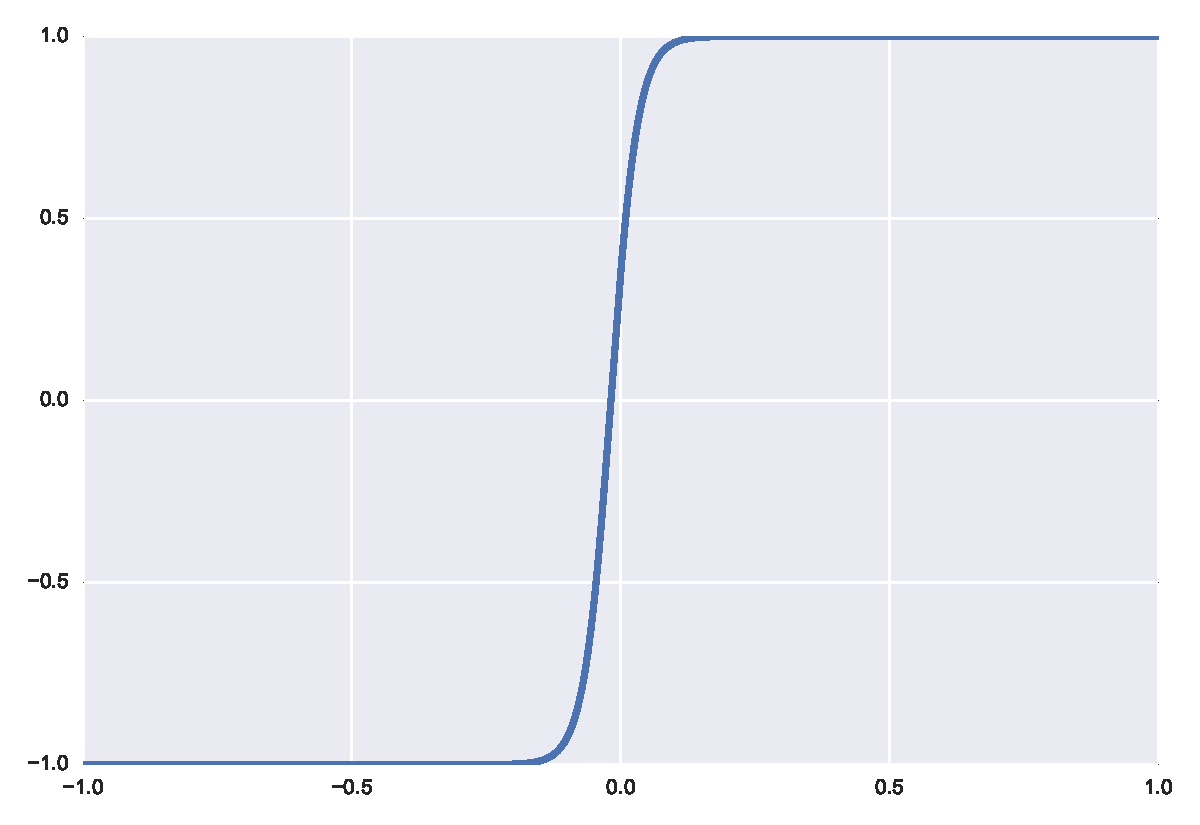
\includegraphics[width=0.7\textwidth]{/h1/dsondak/Research-Notebook/figures/2016/July/burgers_shock.pdf}
  \caption{Illustration of \fenics solution to the steady Burger's equation~\eqref{eq:burgers} using $5000$ finite elements.}
  \label{fig:burgers_shock}
\end{figure}

Next, I need to figure out how to introduce the stabilization parameter into
\fenics.  I'll base this off of Umberto's \fenics implementation of the
stabilization parameter.  Once the stabilization parameter is working, I can 
code up the magnetic field equation, followed by the nondiagonal stabilization
parameter.  Then I will introduce the nondiagonal stabilization parameter and
start compiling the results and the paper.  I will also probably need to
test everything on a two-dimensional problem.  We know that Hartmann flow
doesn't work great.  I'll have to think of another one.

\labday{Tuesday, 19 July, 2016}

\experiment{Combustion Model Inadequacy}
Nearing the end of the calibration of the reduced model.  The hold-up has been invalidating the
reduced model.  The latest results indicate that we may be able to call the calibrated
reduced model inadequate.

\subexperiment{Chemical Kinetics Inadequacy}
It would be nice to invalidate the calibrated reduced model based solely on the 0D reactor.  This has proven difficult
for the five reaction reduced model (see discussion below).  I have tried to invalidate the model with a four
reaction reduced model by removing the three-body reaction.  The algorithmic peformance is much improved (rejection
rates of around $79\%$) and chains that appear stationary.  Figures~\ref{fig:chain_1}-\ref{fig:chain_4} present
the chains from each of the four reactions.
\begin{figure}[h!]
  \centering
  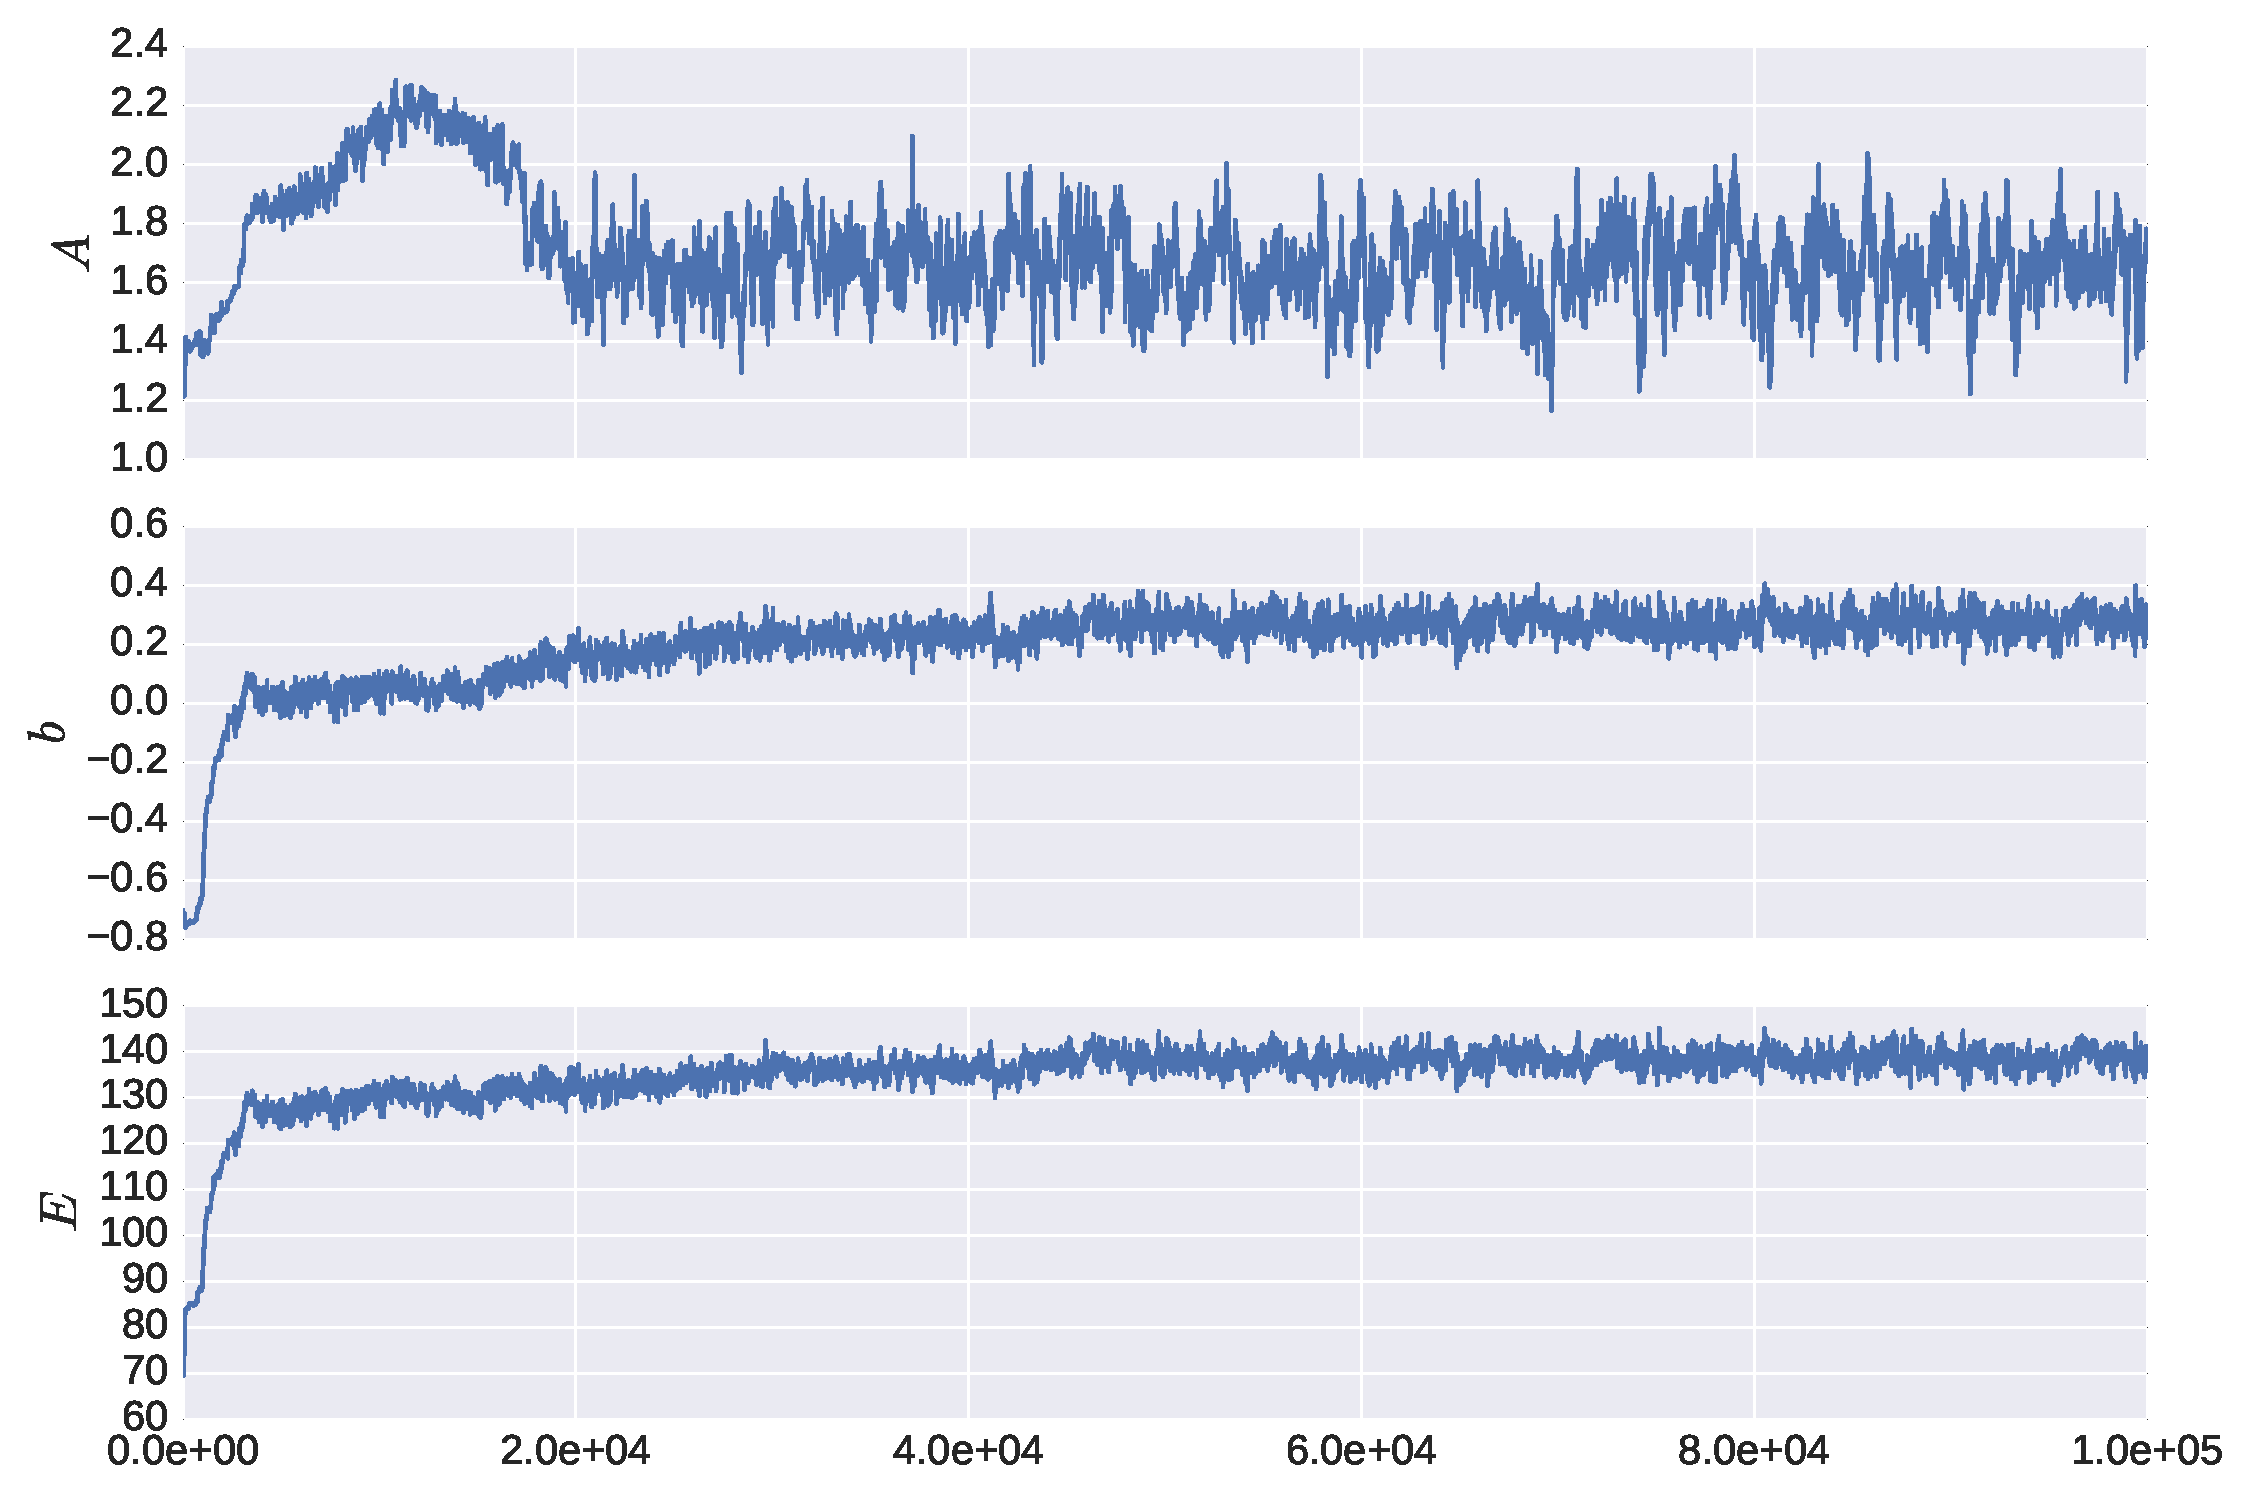
\includegraphics[width=0.7\textwidth]{/h1/dsondak/Research-Notebook/figures/2016/July/reaction0_chain.pdf}
  \caption{Chains from the calibrated Arrhenius parameters for reaction 1.}
  \label{fig:chain_1}
\end{figure}
\begin{figure}[h!]
  \centering
  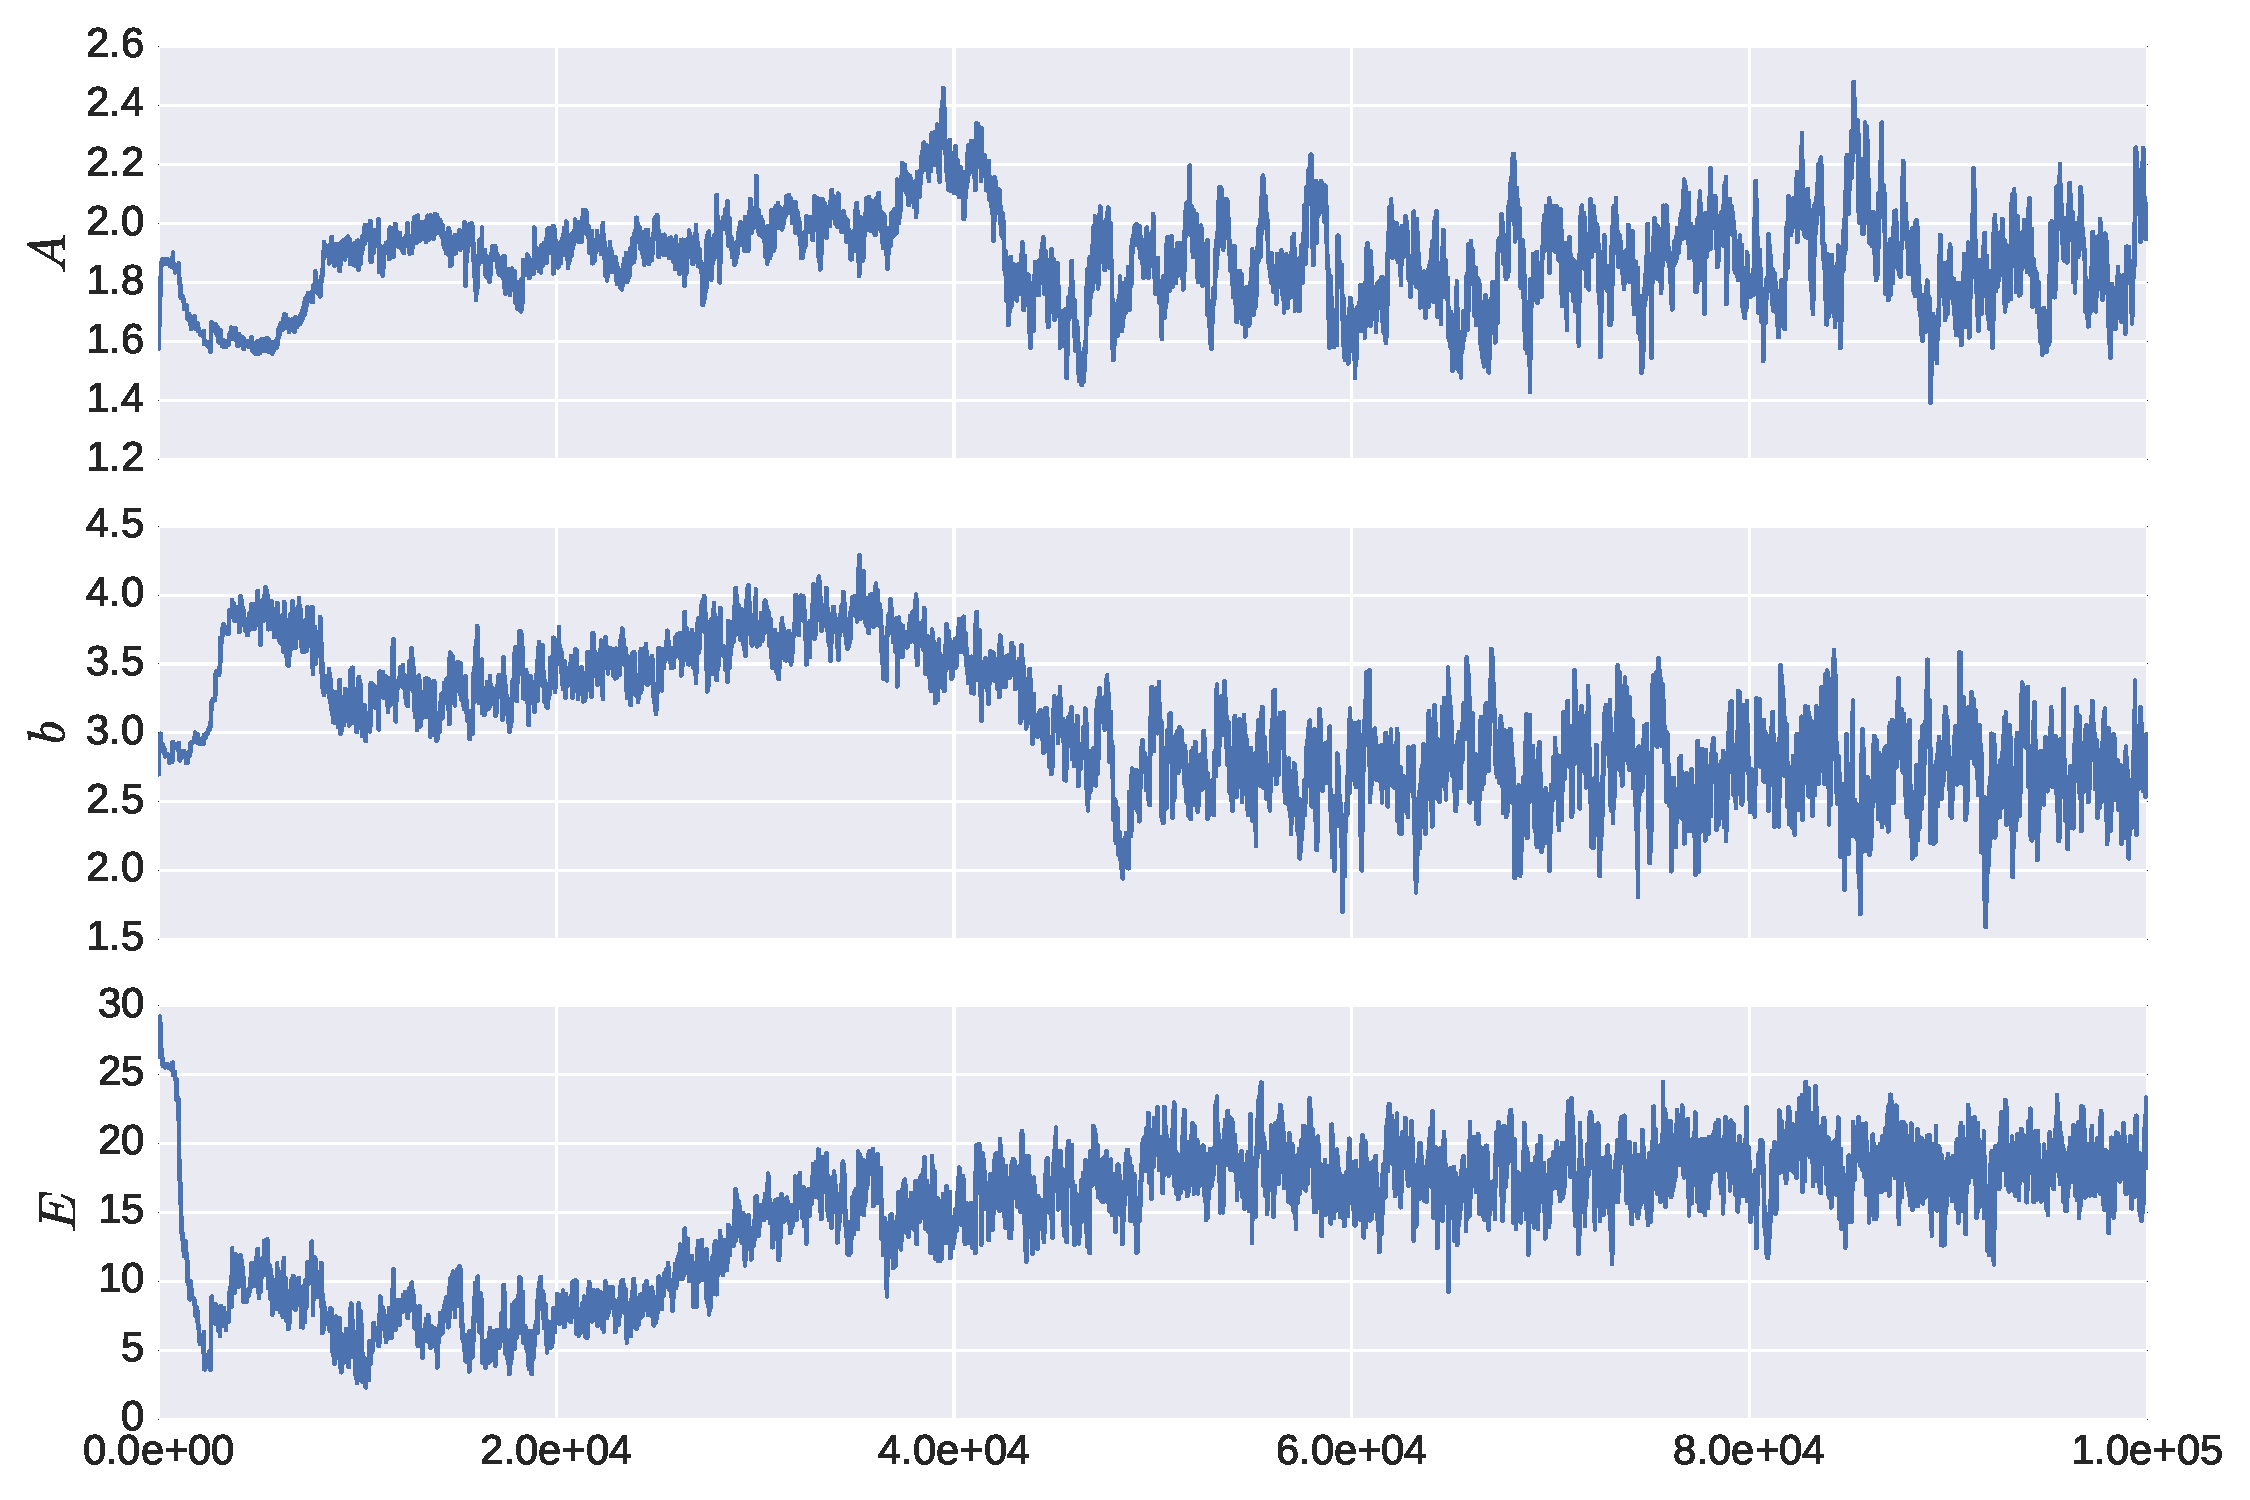
\includegraphics[width=0.7\textwidth]{/h1/dsondak/Research-Notebook/figures/2016/July/reaction1_chain.pdf}
  \caption{Chains from the calibrated Arrhenius parameters for reaction 2.  Note that the modified Arrhenius
           parameter, $b$, was frozen in the simulations even though we present a chain.}
  \label{fig:chain_2}
\end{figure}
\begin{figure}[h!]
  \centering
  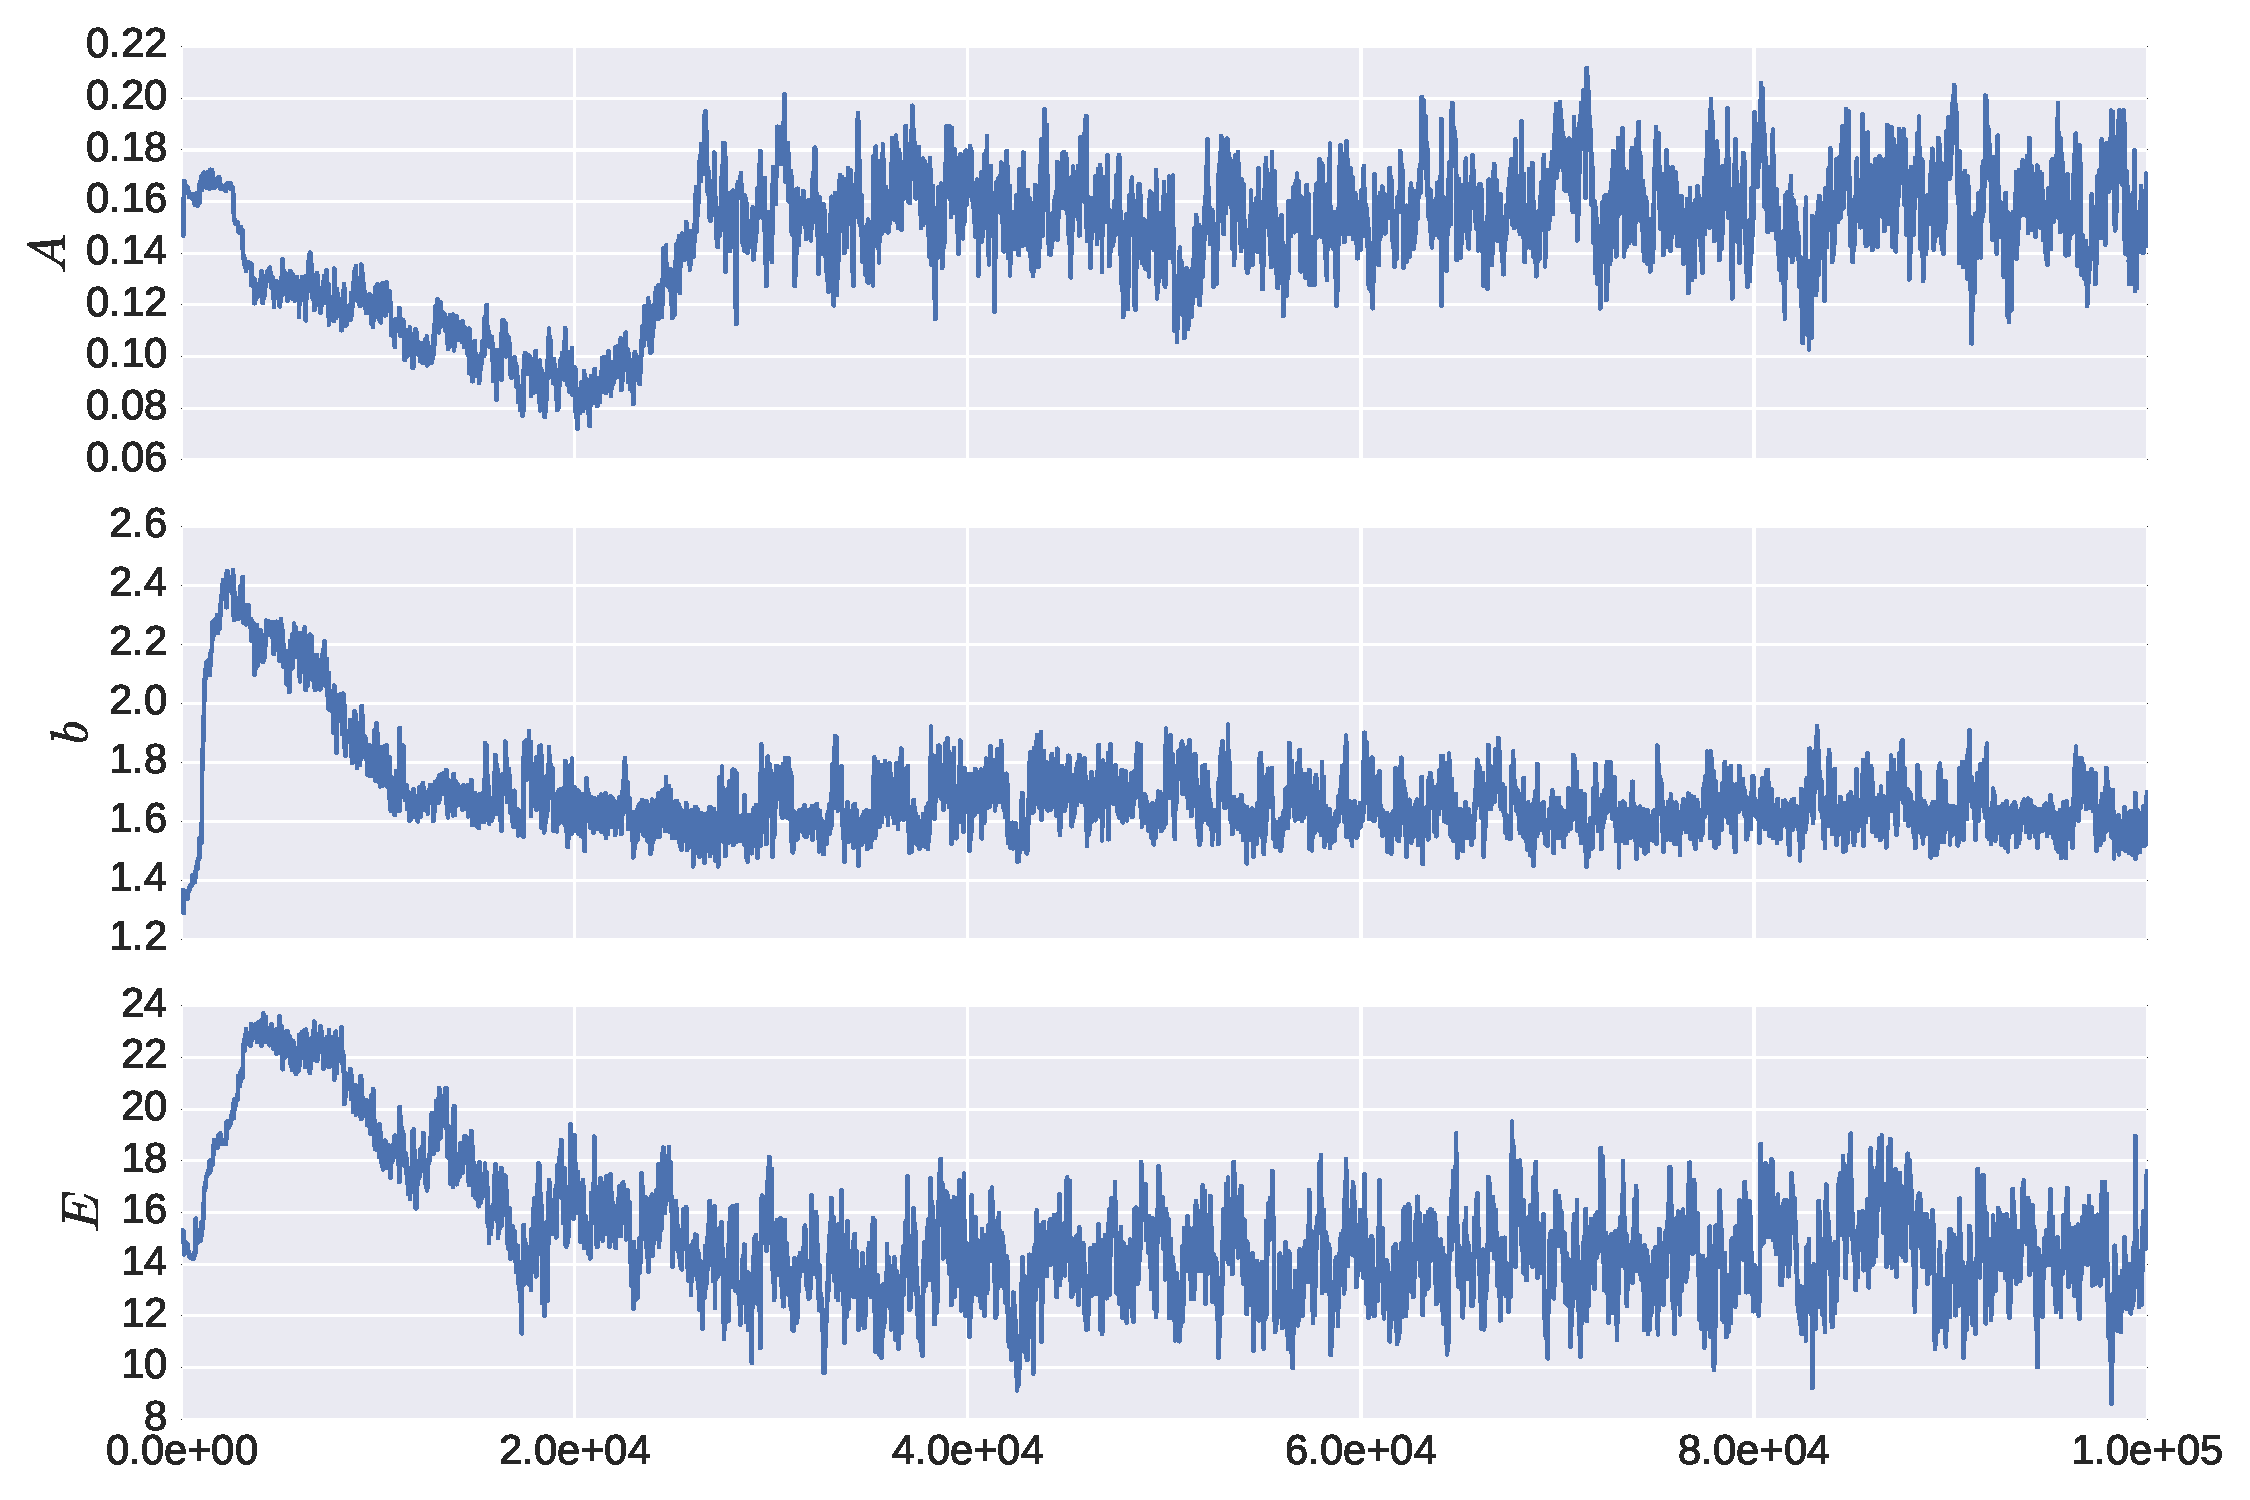
\includegraphics[width=0.7\textwidth]{/h1/dsondak/Research-Notebook/figures/2016/July/reaction2_chain.pdf}
  \caption{Chains from the calibrated Arrhenius parameters for reaction 3.}
  \label{fig:chain_3}
\end{figure}
\begin{figure}[h!]
  \centering
  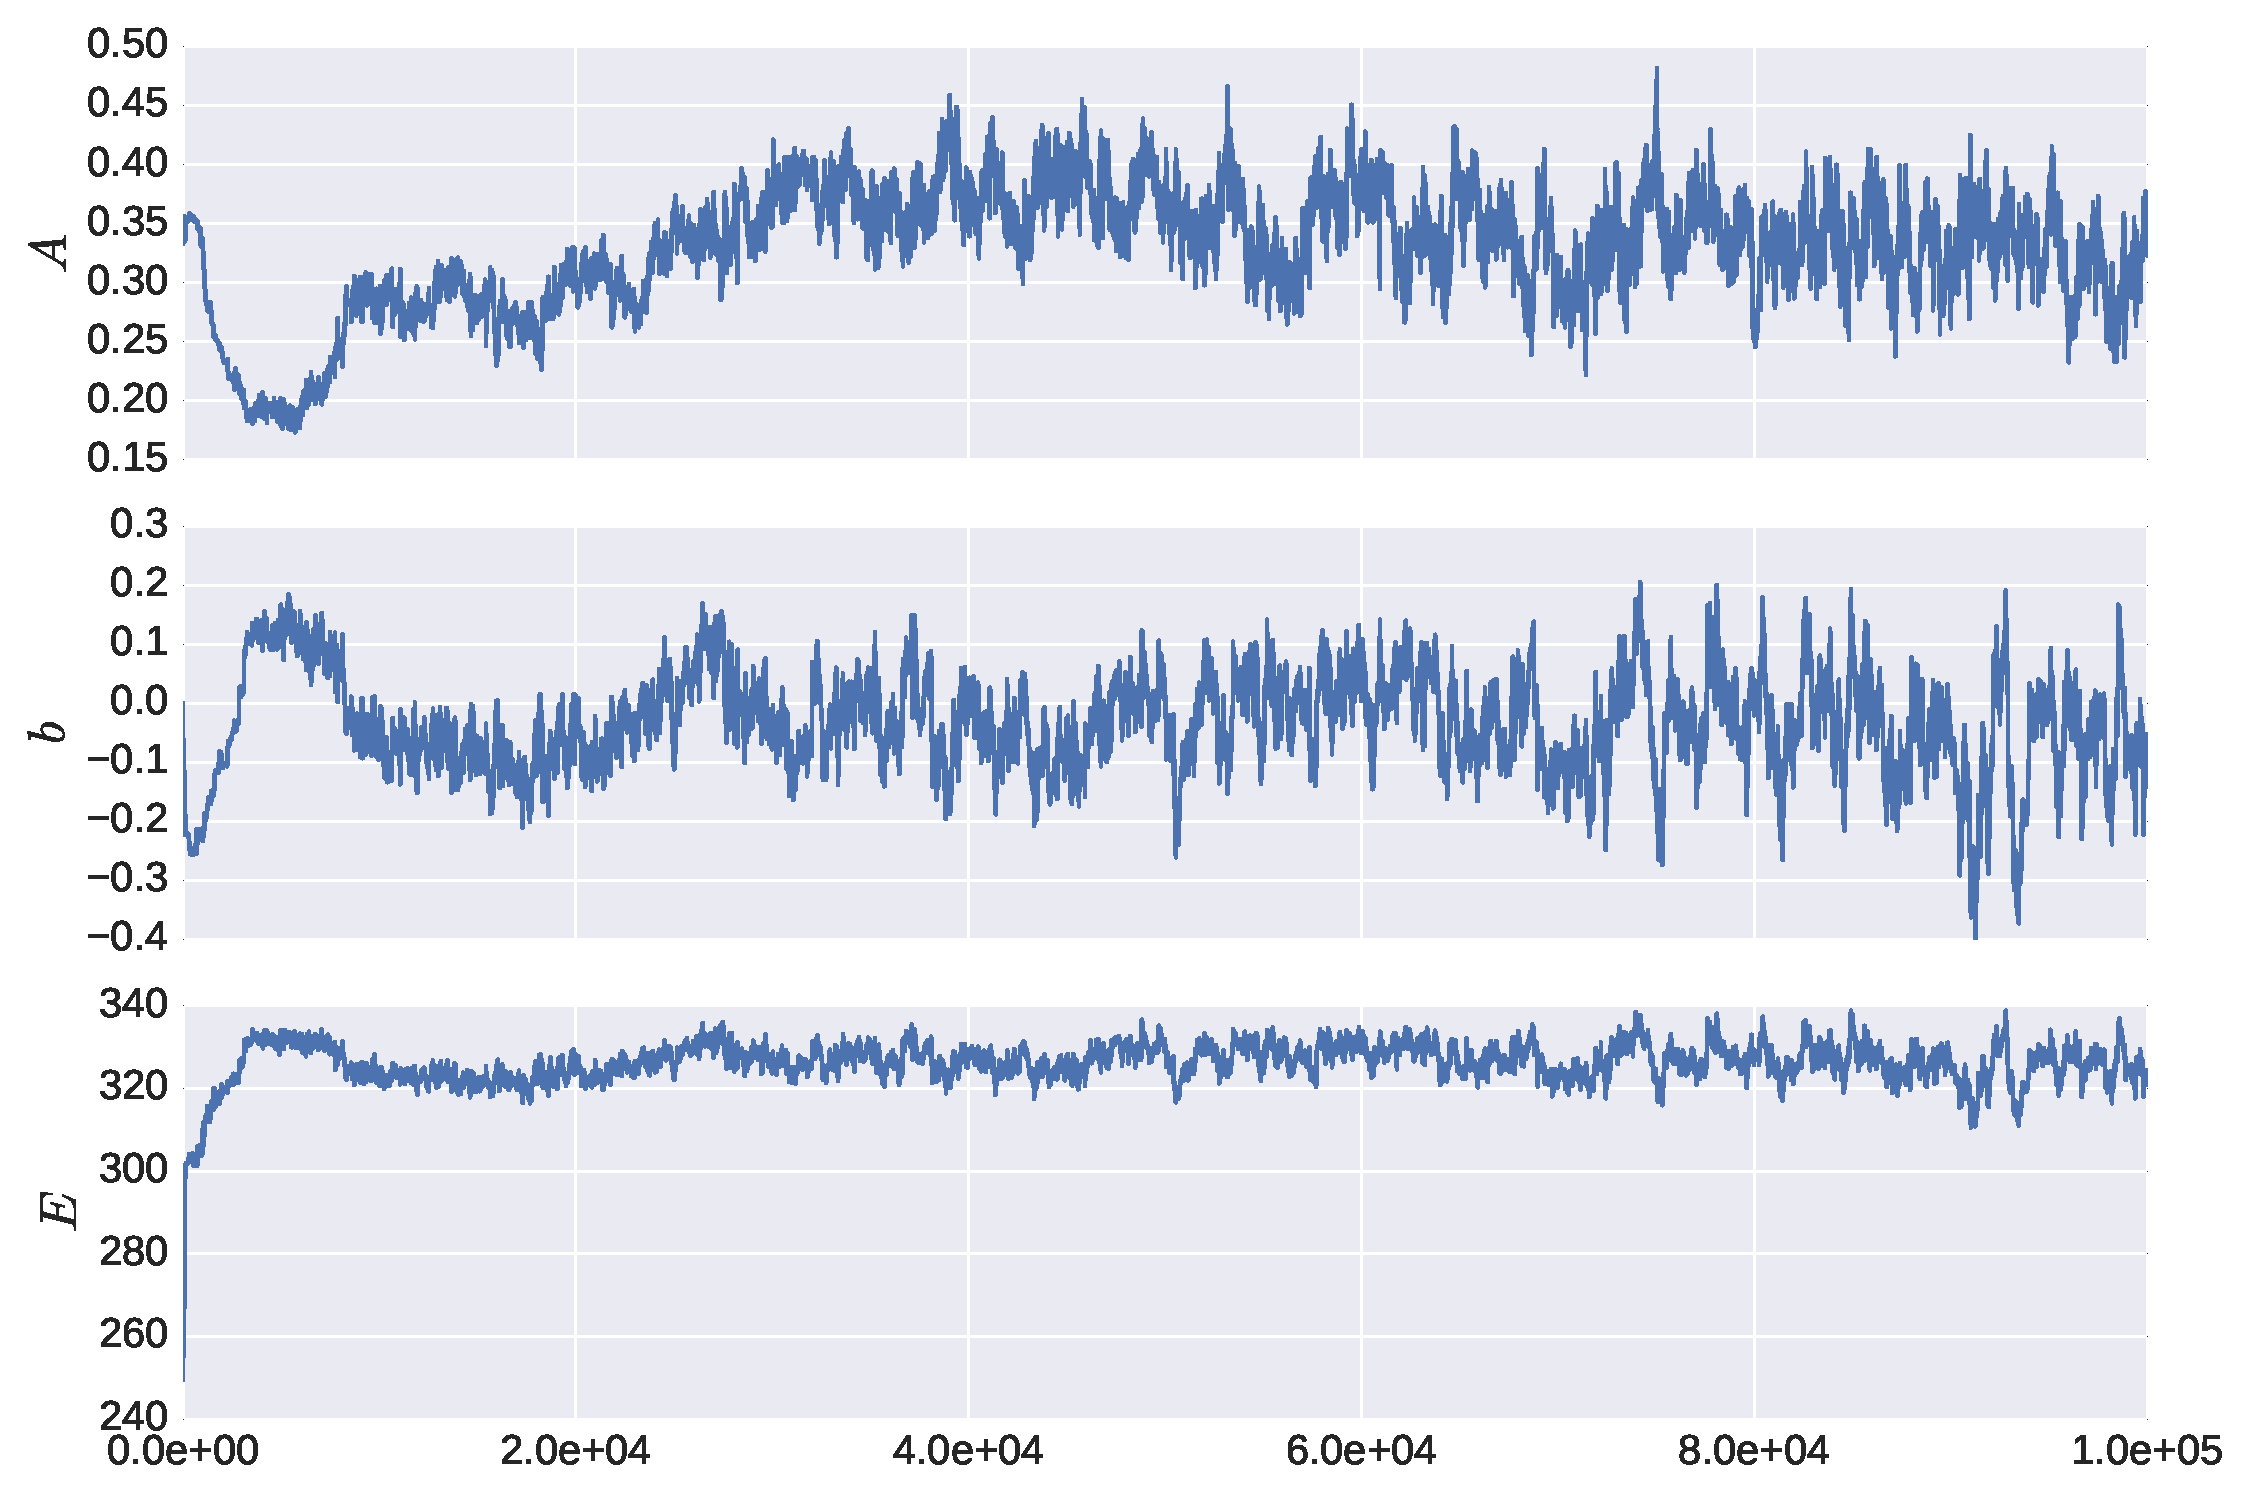
\includegraphics[width=0.7\textwidth]{/h1/dsondak/Research-Notebook/figures/2016/July/reaction3_chain.pdf}
  \caption{Chains from the calibrated Arrhenius parameters for reaction 4.}
  \label{fig:chain_4}
\end{figure}
We also provide the posterior and prior distributions for each parameter in Figures~\ref{fig:dist_1}-\ref{fig:dist_4}.  
Note that the modified Arrhenius parameter, $b$, was not actually calibrated.  It was frozen during the simulation.
\begin{figure}[h!]
  \centering
  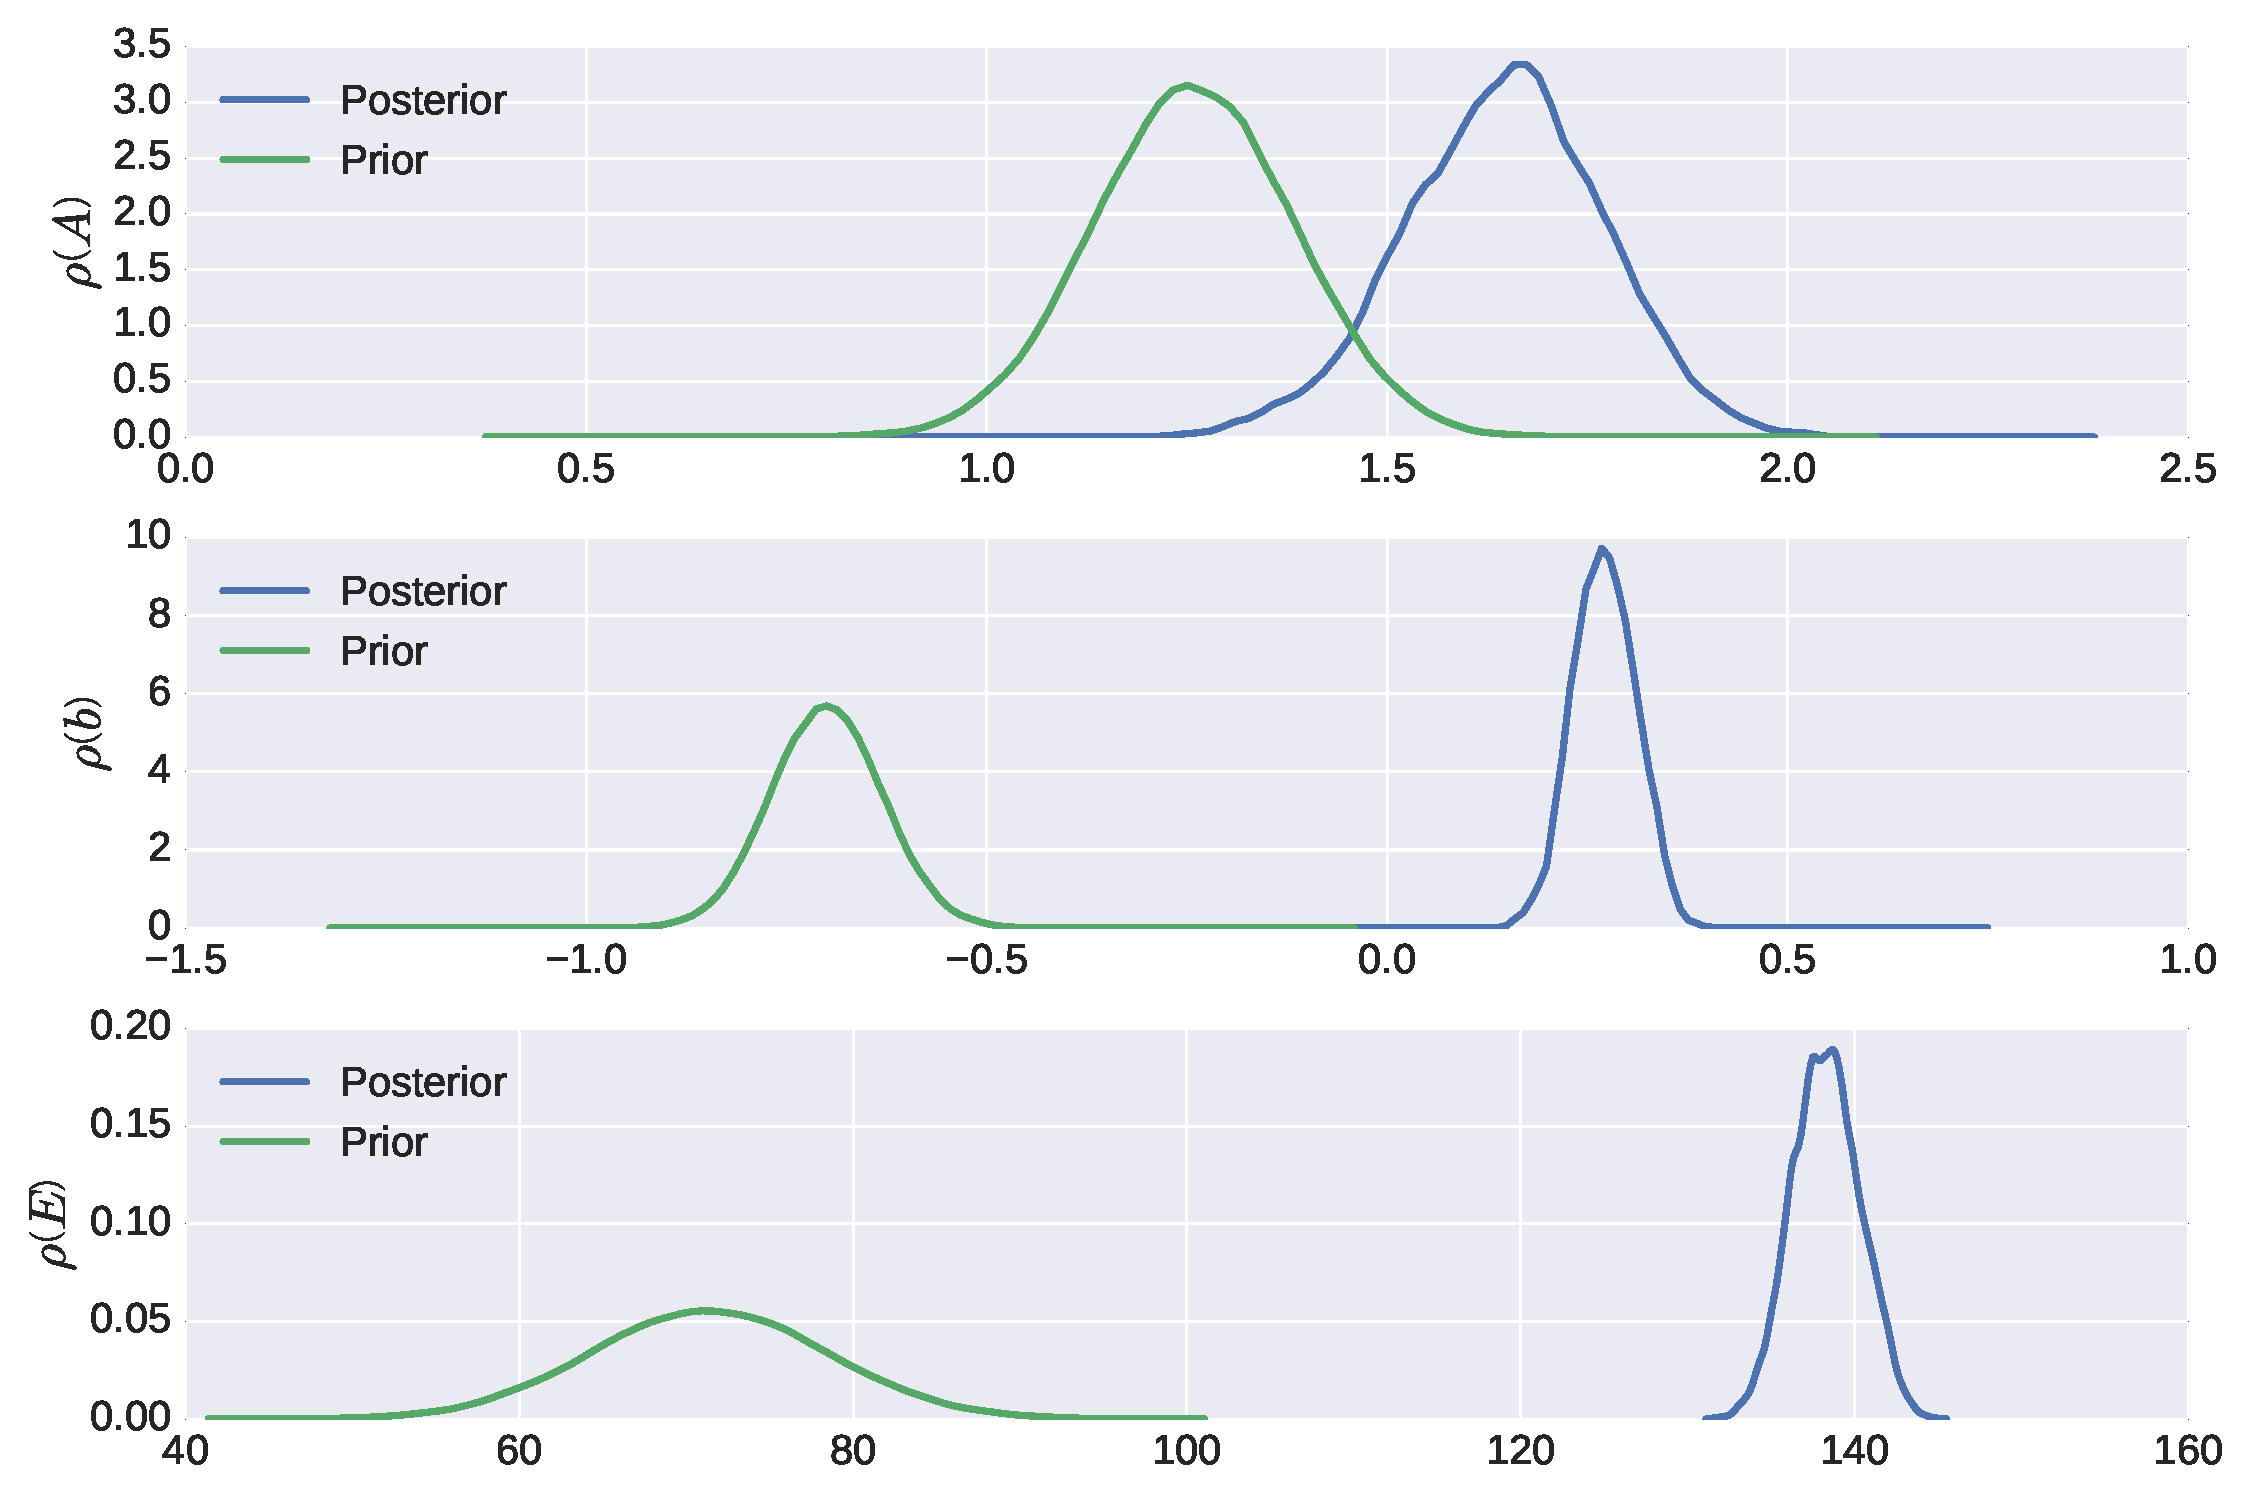
\includegraphics[width=0.7\textwidth]{/h1/dsondak/Research-Notebook/figures/2016/July/reaction0_dist.pdf}
  \caption{Posterior and prior distributions from the calibrated Arrhenius parameters for reaction 1.}
  \label{fig:dist_1}
\end{figure}
\begin{figure}[h!]
  \centering
  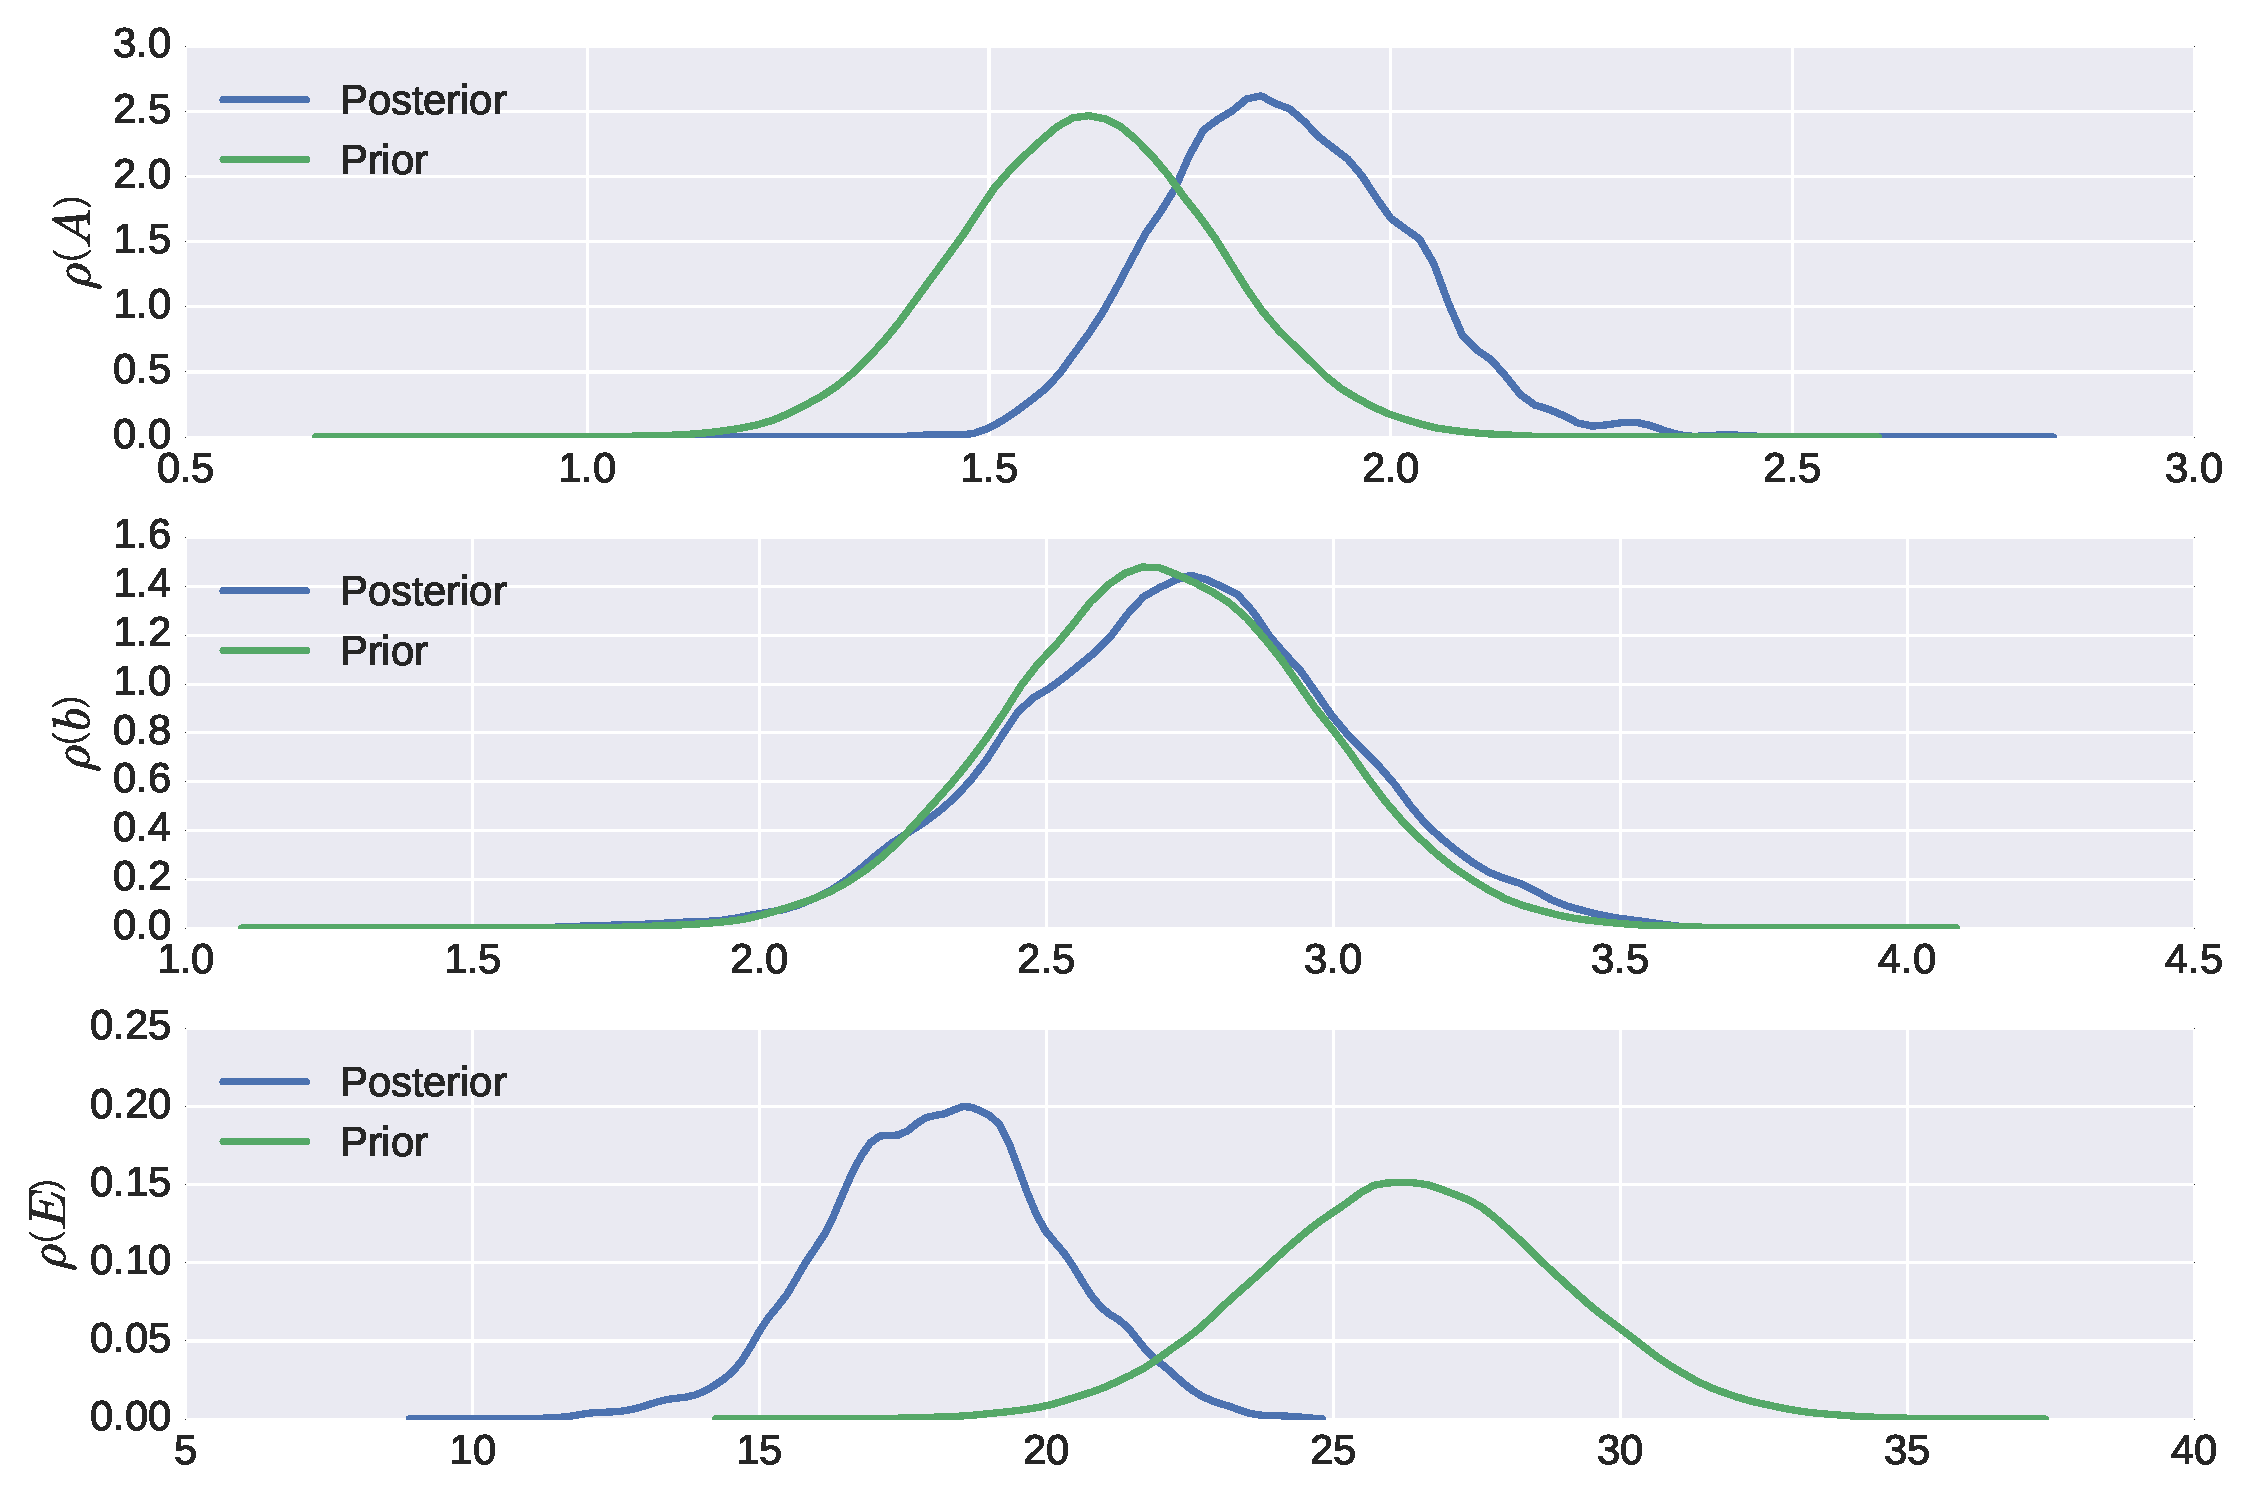
\includegraphics[width=0.7\textwidth]{/h1/dsondak/Research-Notebook/figures/2016/July/reaction1_dist.pdf}
  \caption{Posterior and prior distributions from the calibrated Arrhenius parameters for reaction 2.  Note that the modified Arrhenius
           parameter, $b$, was frozen in the simulations even though we present a chain.}
  \label{fig:dist_2}
\end{figure}
\begin{figure}[h!]
  \centering
  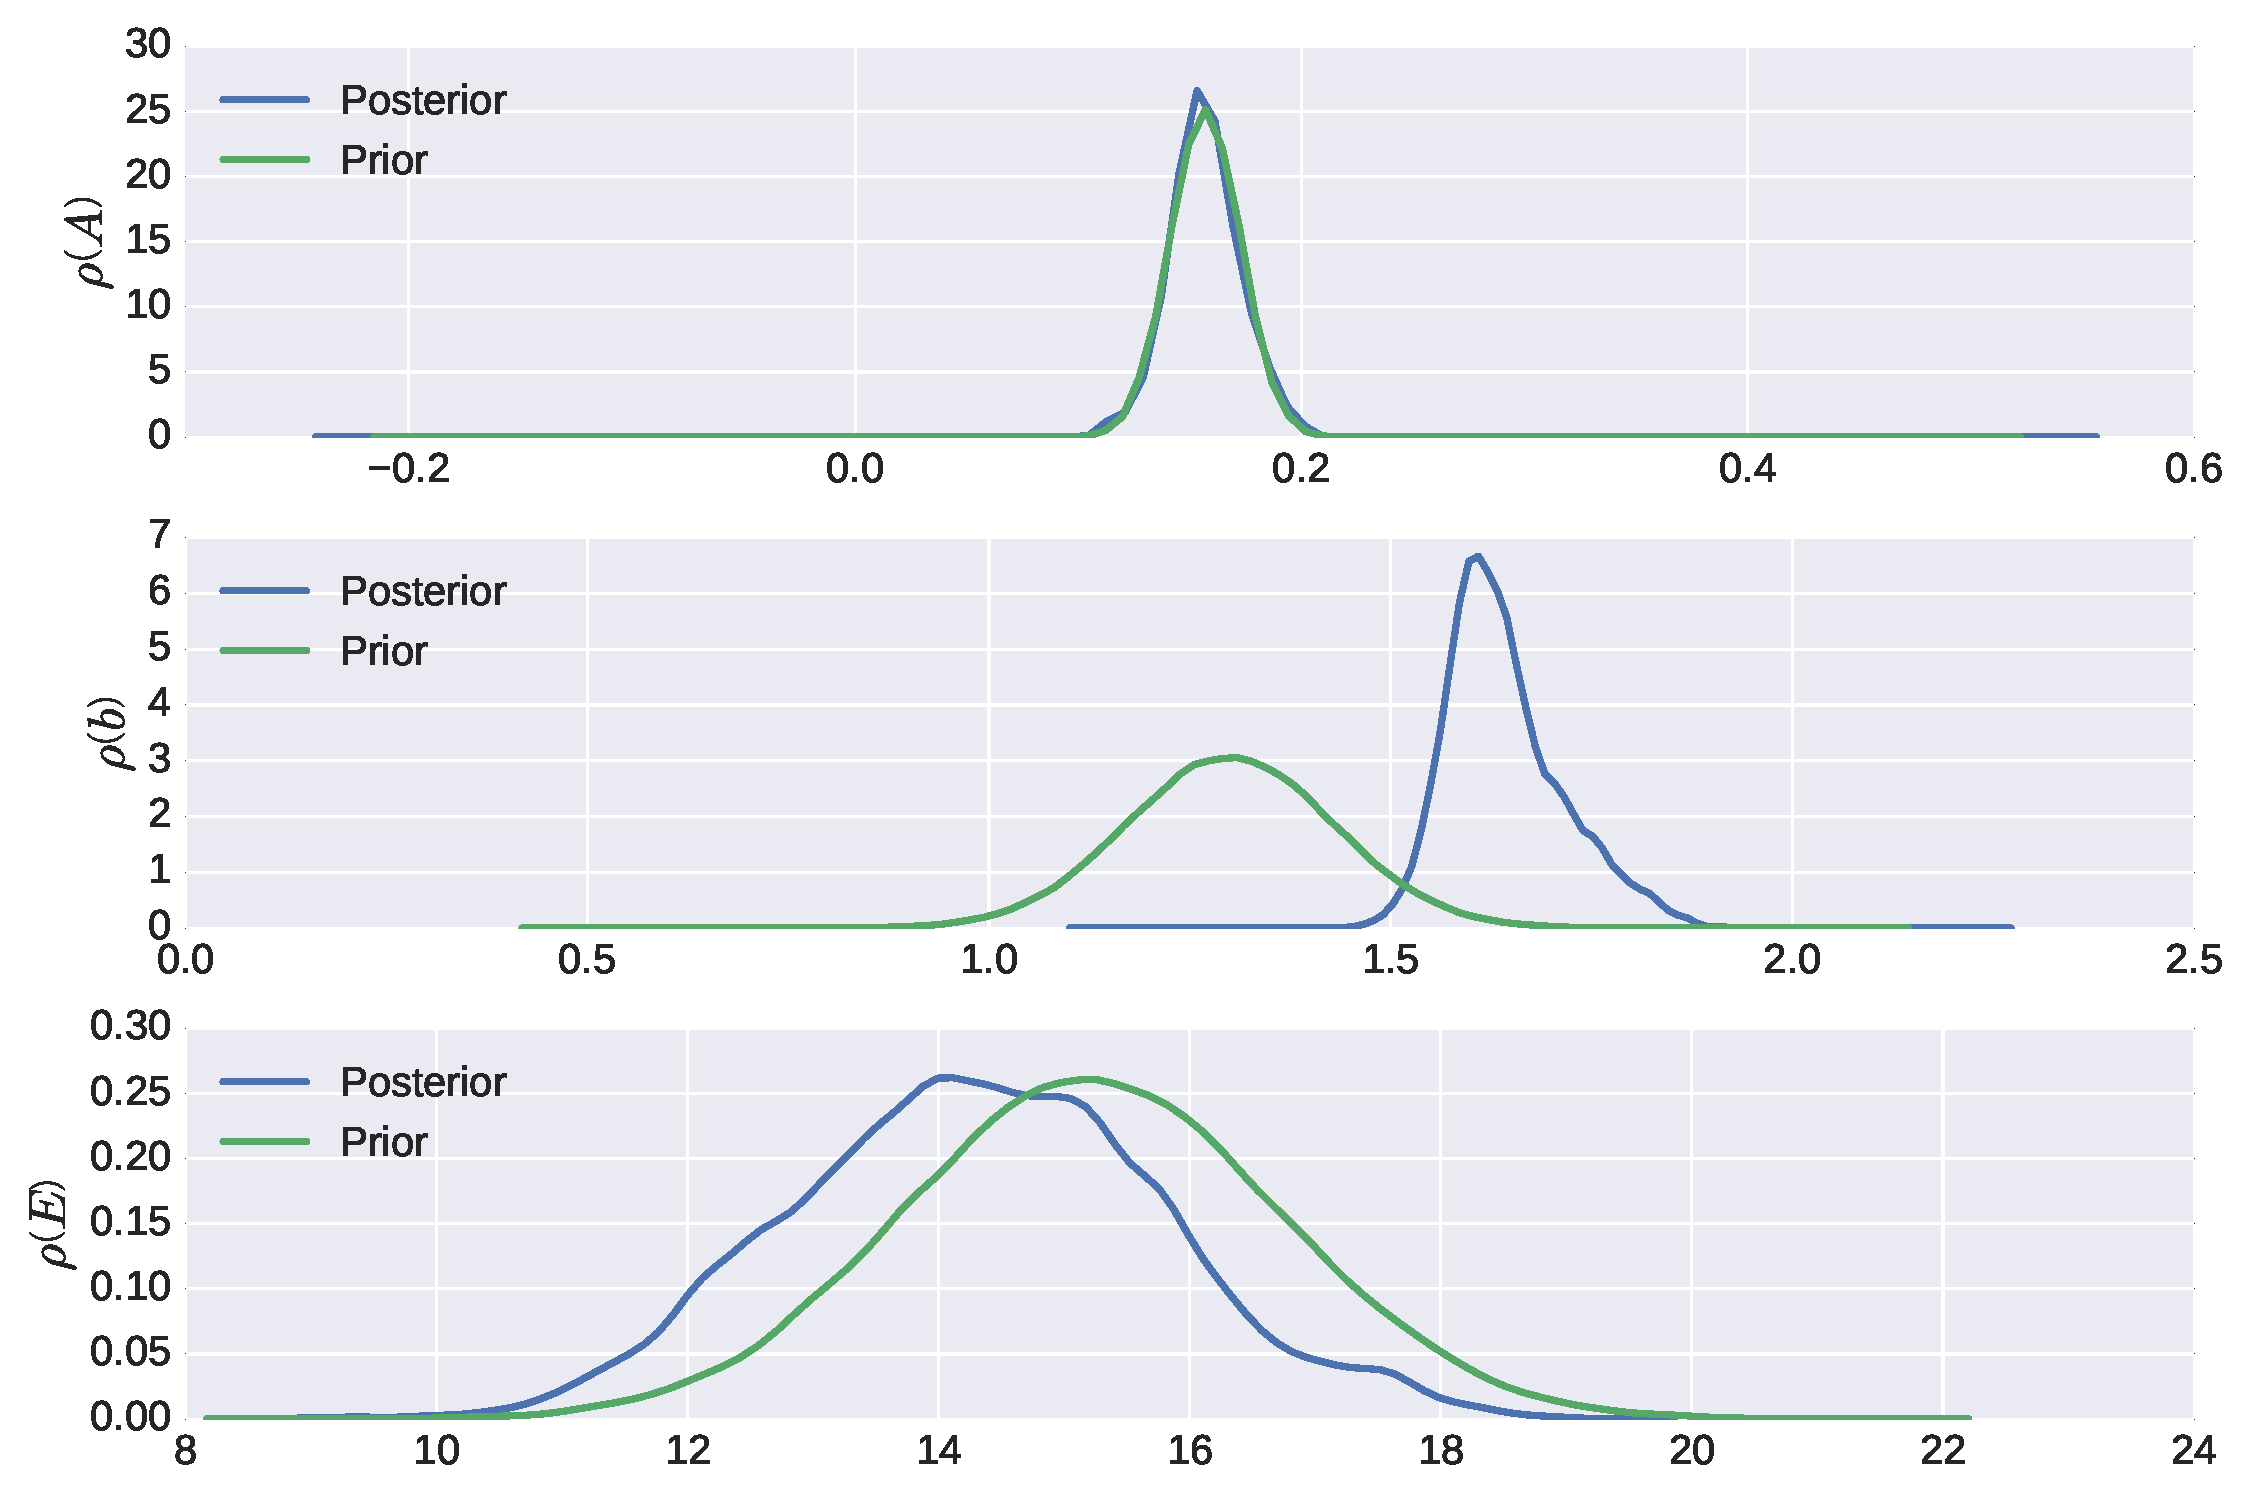
\includegraphics[width=0.7\textwidth]{/h1/dsondak/Research-Notebook/figures/2016/July/reaction2_dist.pdf}
  \caption{Posterior and prior distributions from the calibrated Arrhenius parameters for reaction 3.}
  \label{fig:dist_3}
\end{figure}
\begin{figure}[h!]
  \centering
  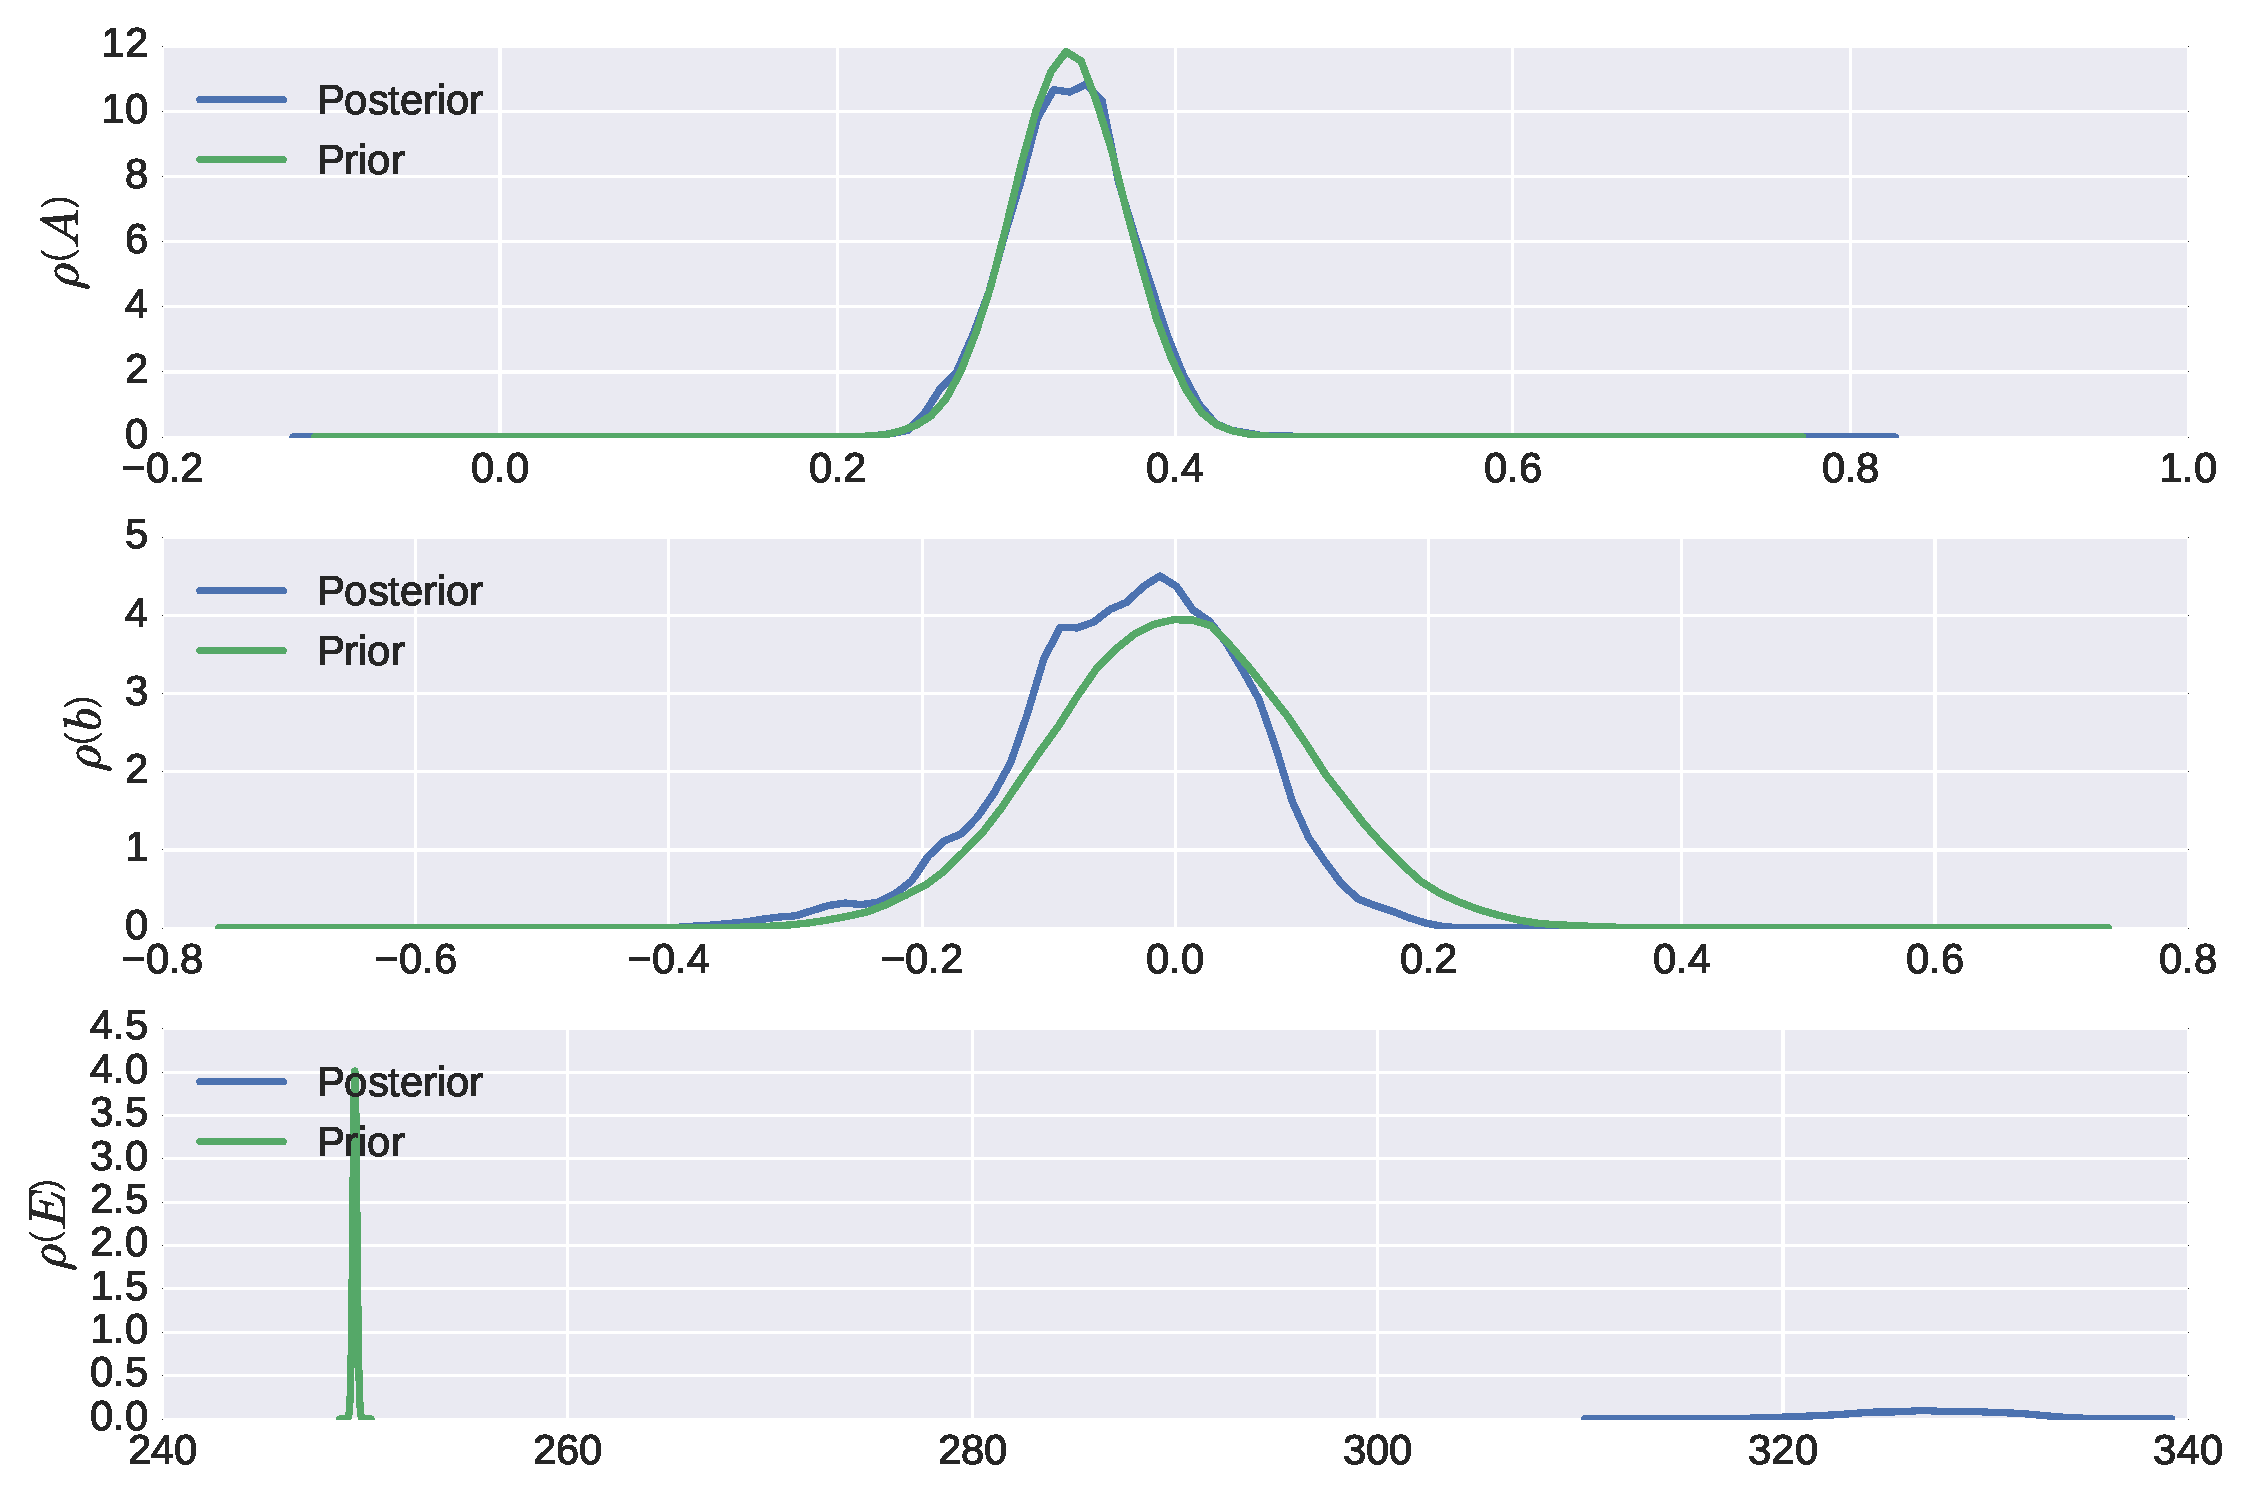
\includegraphics[width=0.7\textwidth]{/h1/dsondak/Research-Notebook/figures/2016/July/reaction3_dist.pdf}
  \caption{Posterior and prior distributions from the calibrated Arrhenius parameters for reaction 4.}
  \label{fig:dist_4}
\end{figure}
It appears that we are learning quite a bit about a few parameters.  The maximum likelihood and MAP point
were obtained from the chains and the forward problem was run at each of these parameter sets.  The 
problem was also run at the nominal parameter set.  Results were compared with the detailed model and are
shown in Figure~\ref{fig:four_rxn_inad}.
\begin{figure}[h!]
  \centering
  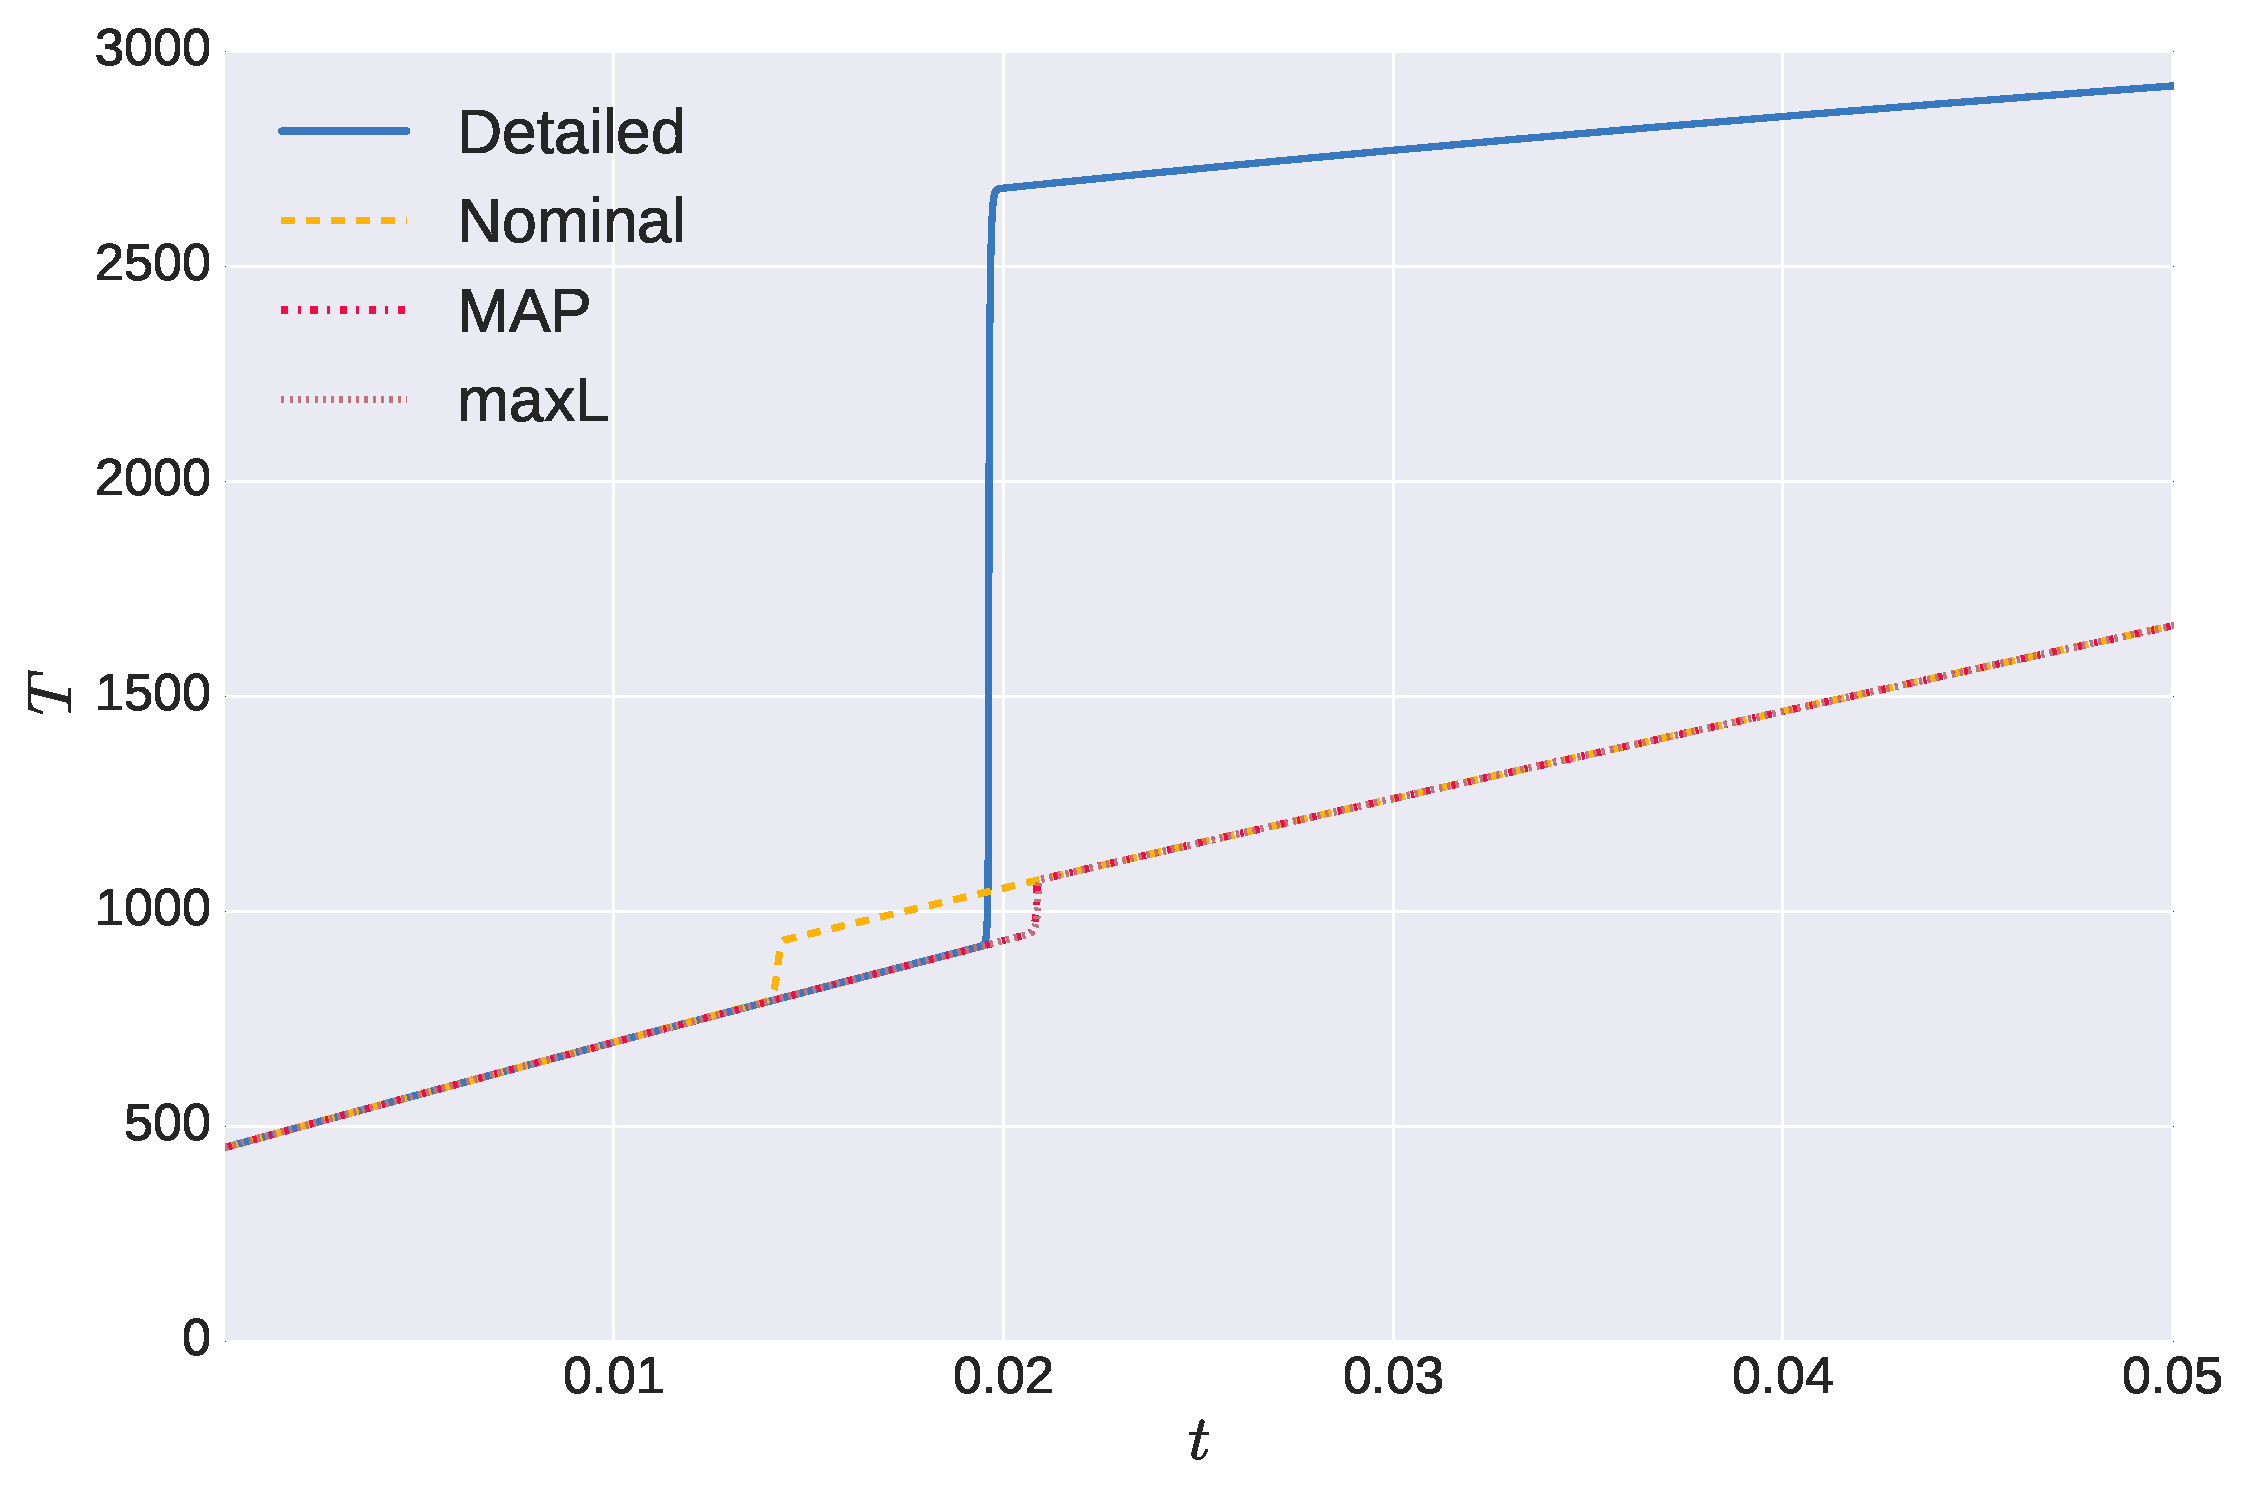
\includegraphics[width=0.7\textwidth]{/h1/dsondak/Research-Notebook/figures/2016/July/Toft_four_rxn_inad.pdf}
  \caption{Time evolution of the temperature.  Comparisons are made between the four reaction reduced model
           for three different parameter sets and the detailed model.  Results are shown at $\phi=1$ which
           is the equivalence ratio at which the data was calibrated.}
  \label{fig:four_rxn_inad}
\end{figure}
Even after calibration, the four reaction model is inadequate.  This may provide a simple route to helping
Rebecca get her stuff going again.  I'll need to calibrate the stochastic operator on this problem and then
see how things look.  For now, I need to get the stochastic operator up and running.

\subexperiment{Diffusion Flame}
The diffusion flame will eventually be used to build up a flamelet library.  For now, I'm just using it to
see if it helps us invalidate the five reaction reduced mechanism.  Figures~\ref{fig:T_Z}-\ref{fig:H2_x} were generated
from samples of the five reaction reduced mechanism.
\begin{figure}[h!]
  \centering
  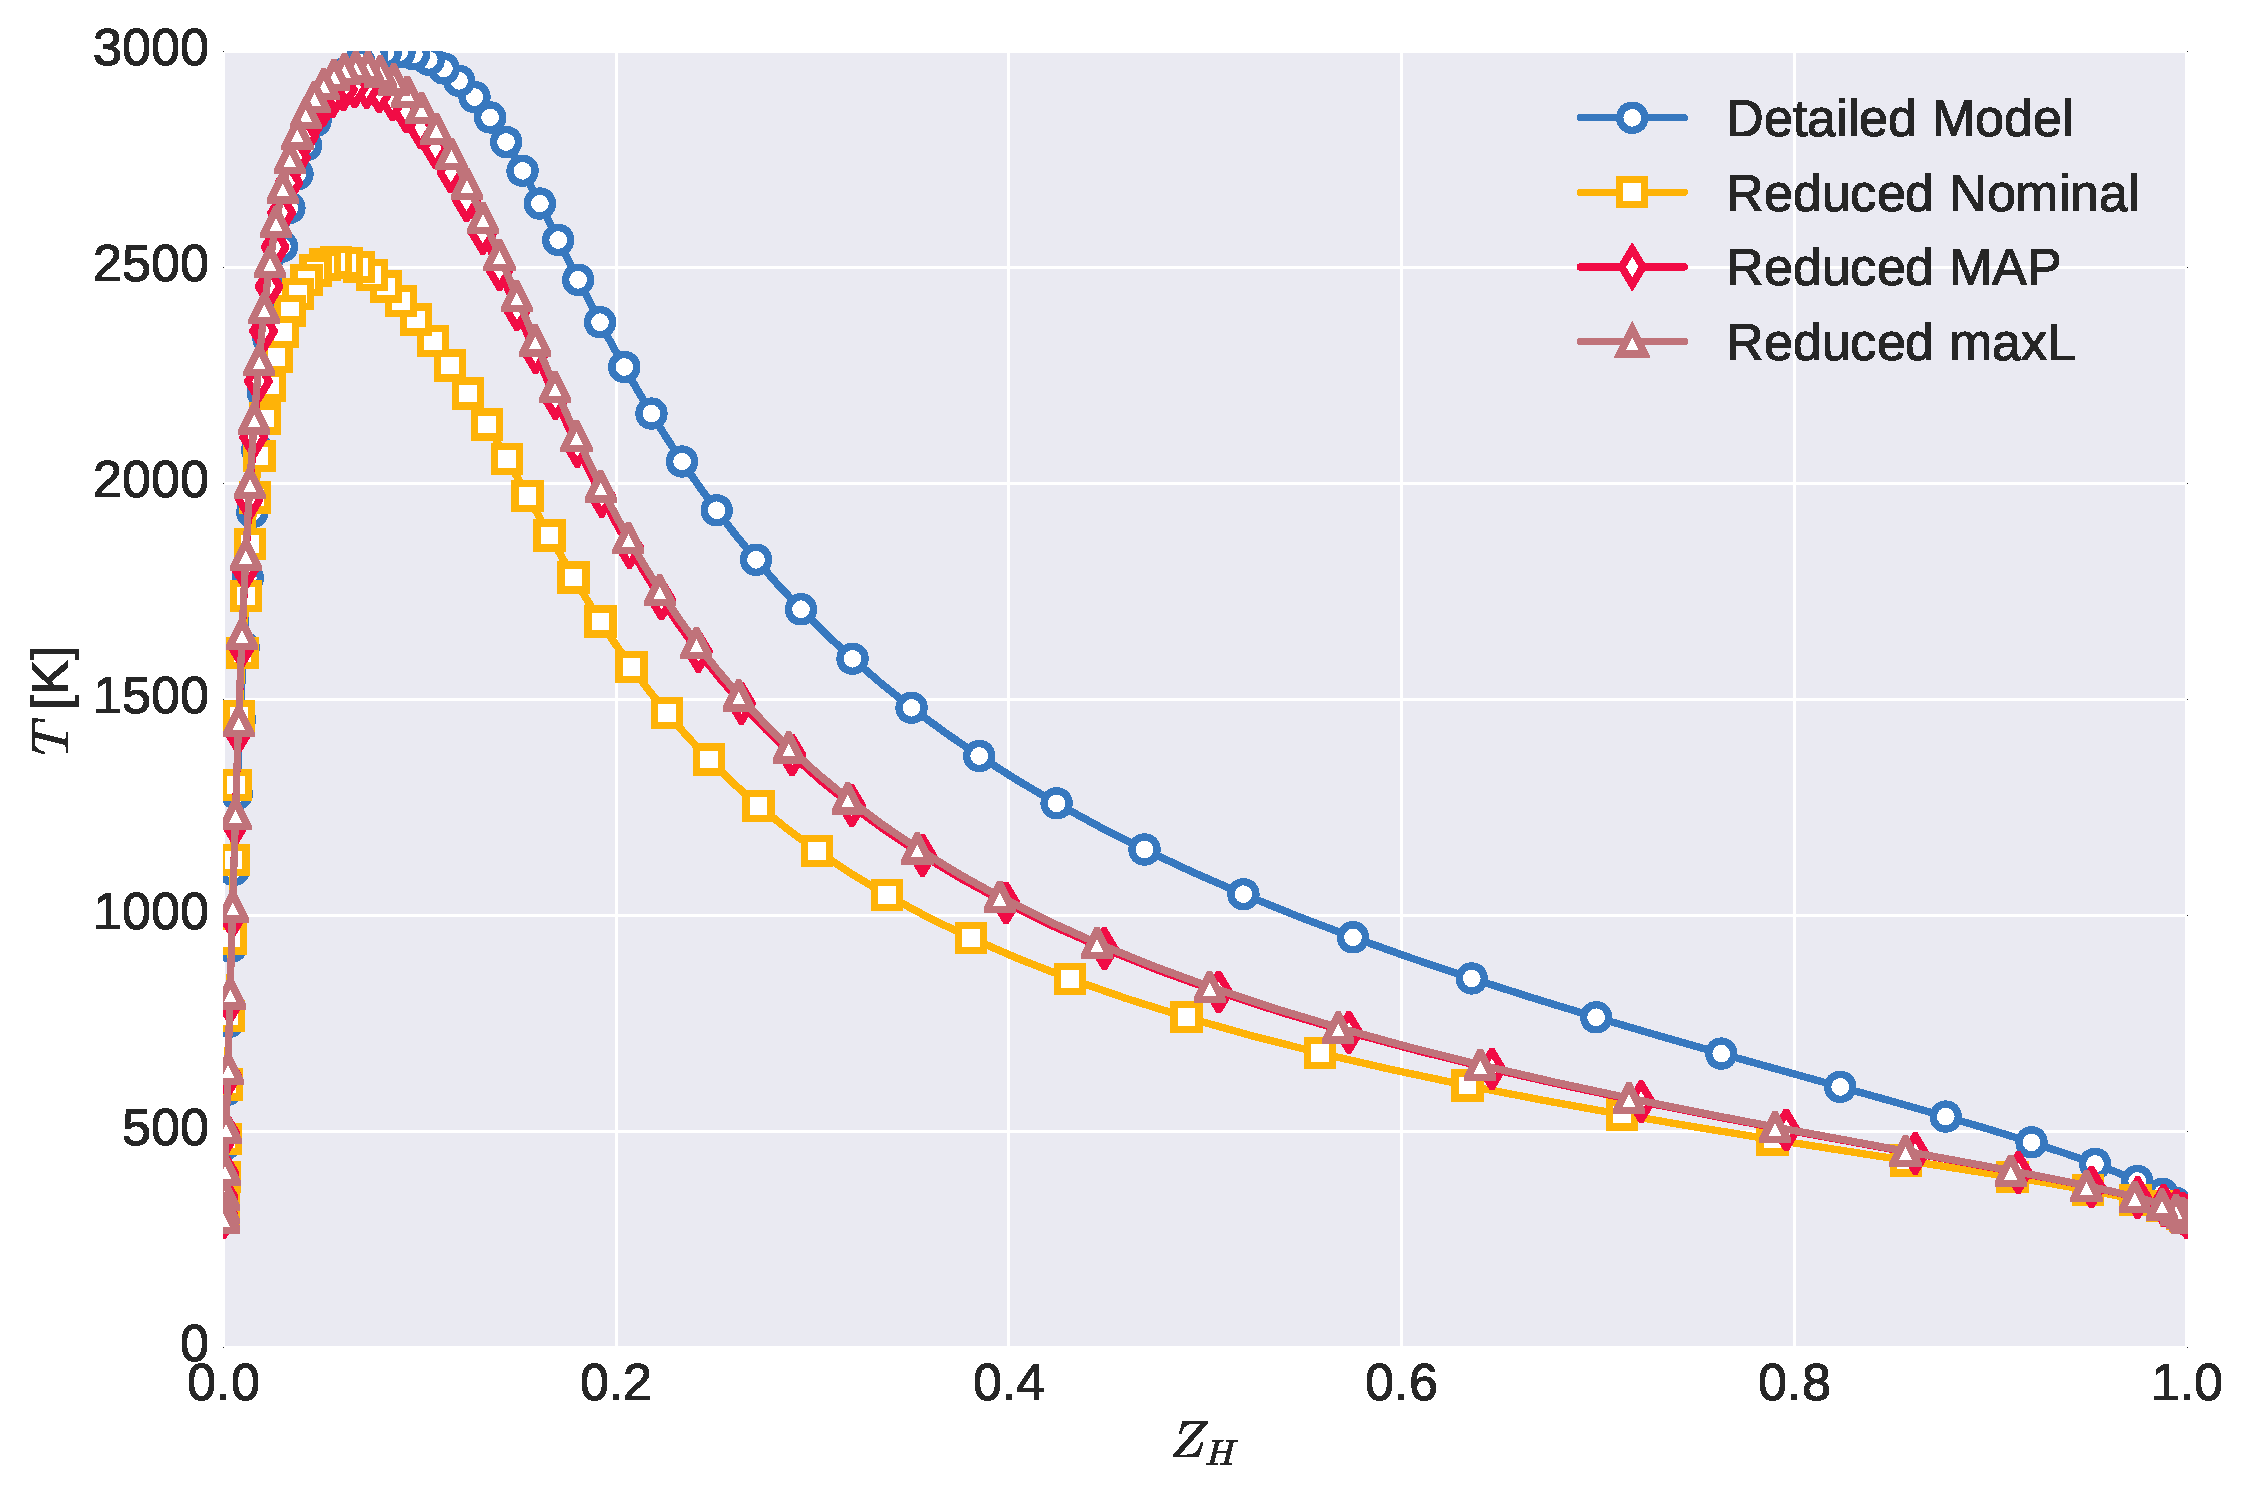
\includegraphics[width=0.7\textwidth]{/h1/dsondak/Research-Notebook/figures/2016/July/T_Z.pdf}
  \caption{Temperature as a function of mixture fraction.}
  \label{fig:T_Z}
\end{figure}
\begin{figure}[h!]
  \centering
  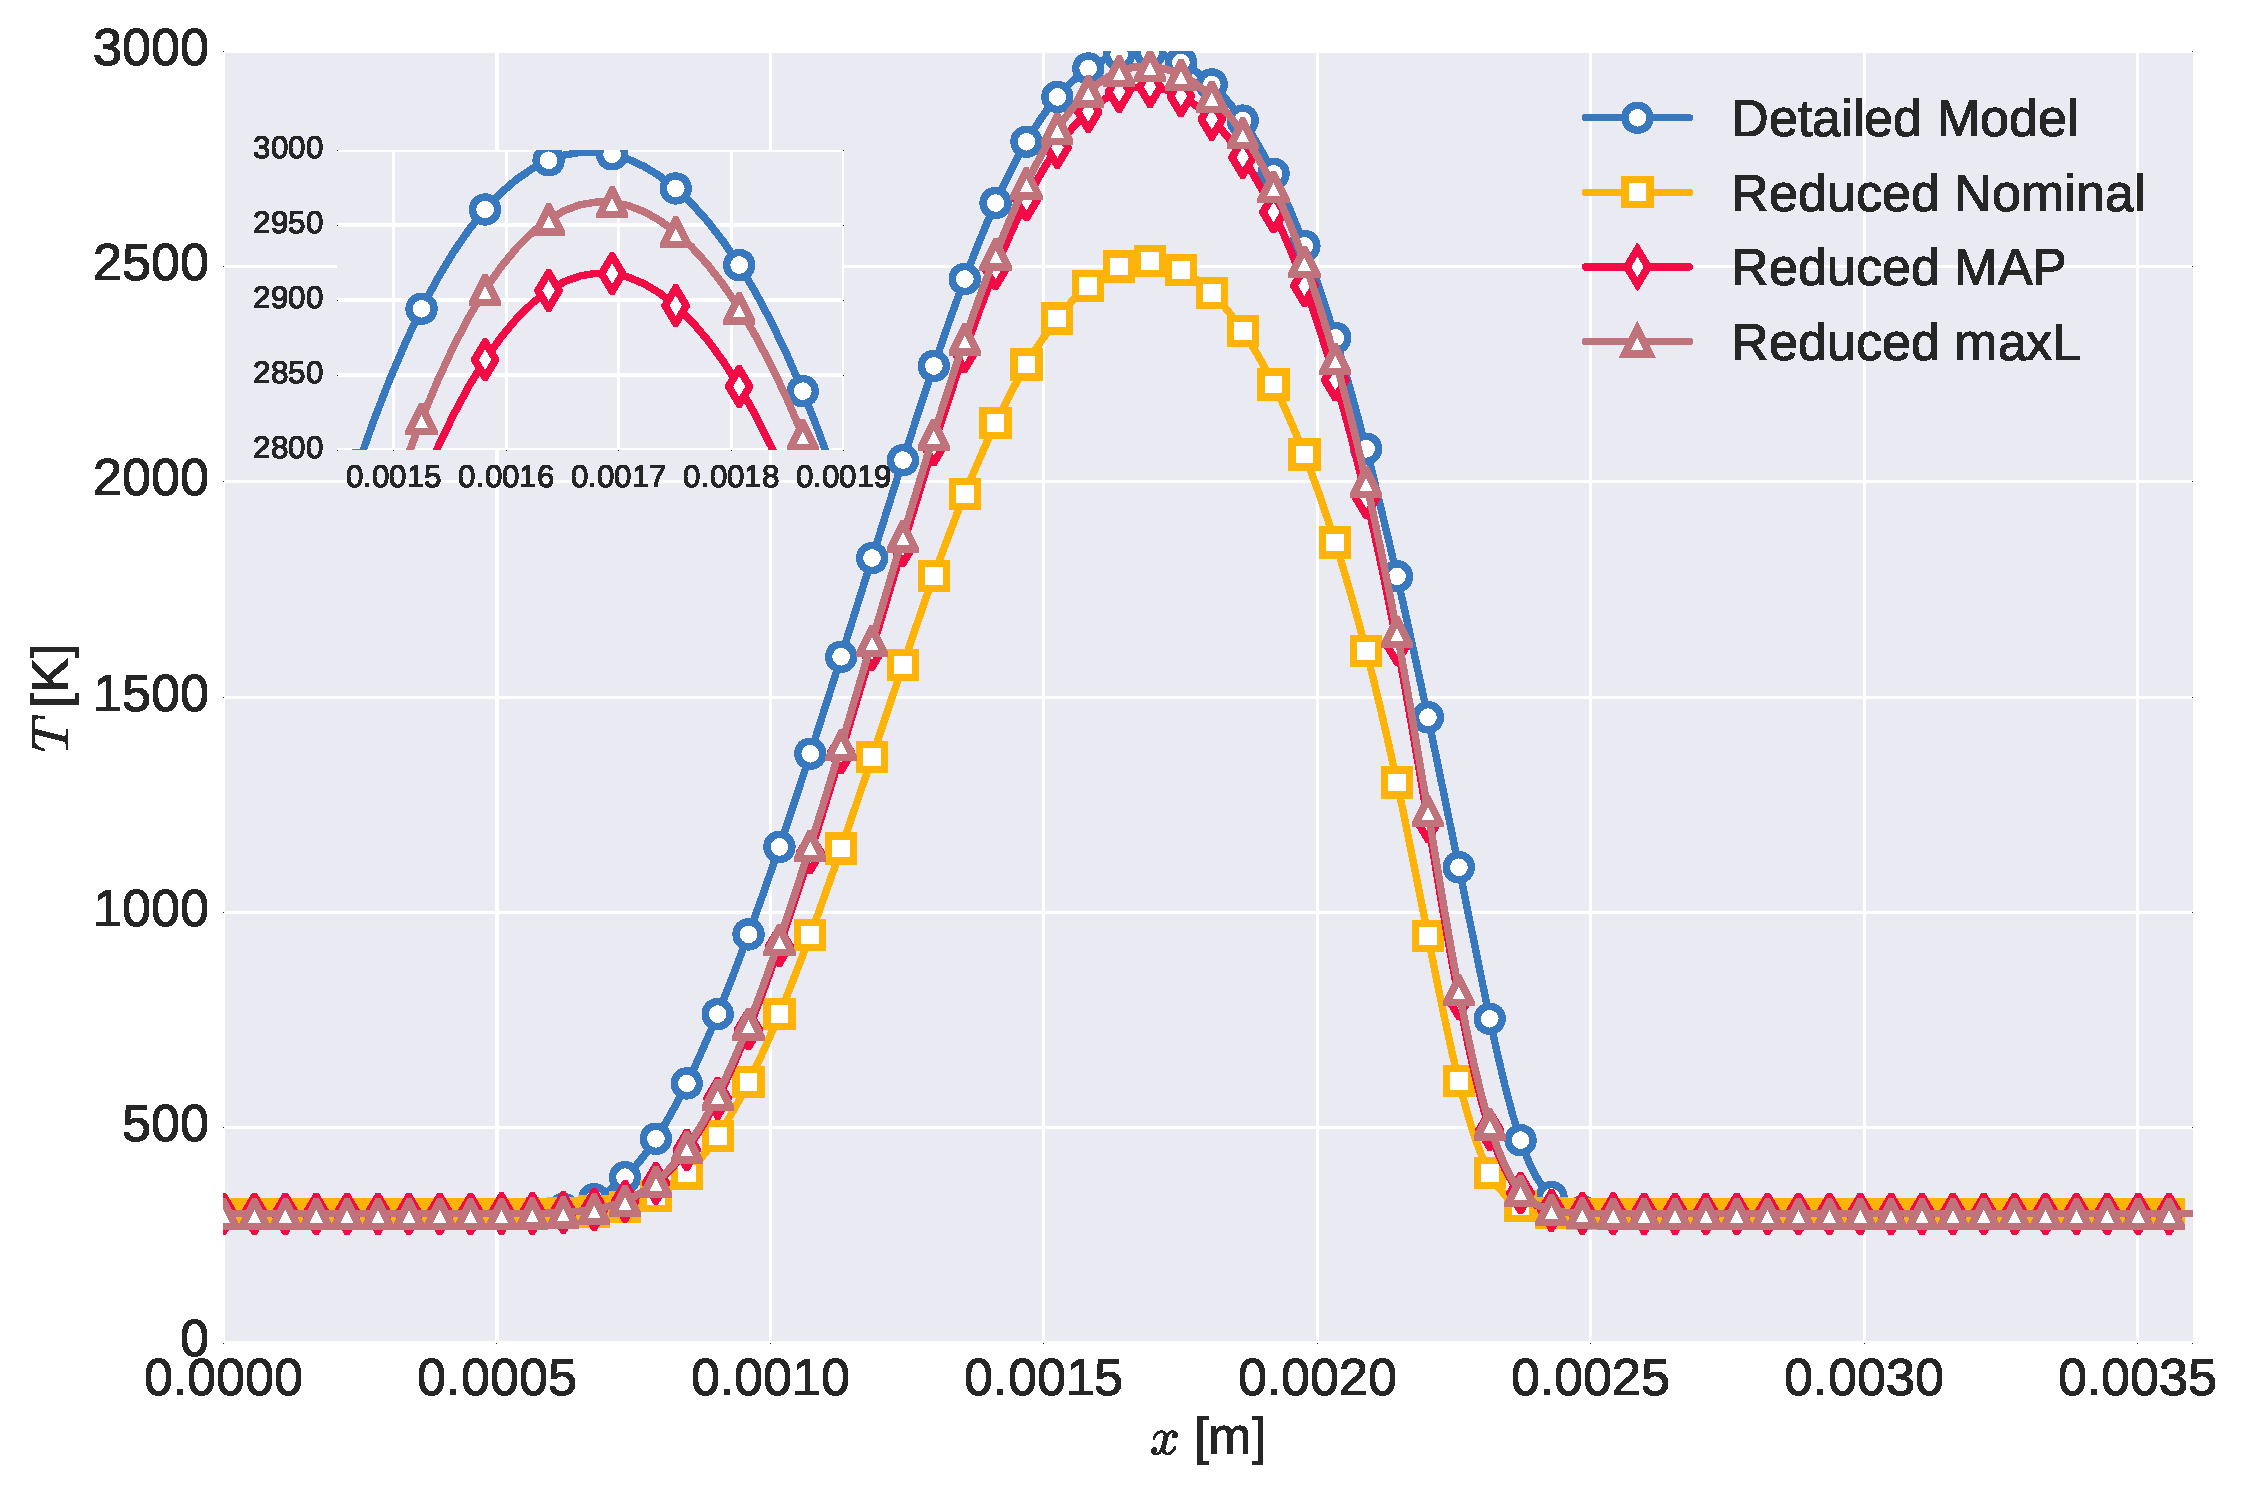
\includegraphics[width=0.7\textwidth]{/h1/dsondak/Research-Notebook/figures/2016/July/T_x.pdf}
  \caption{Temperature as a function of space.}
  \label{fig:T_x}
\end{figure}
\begin{figure}[h!]
  \centering
  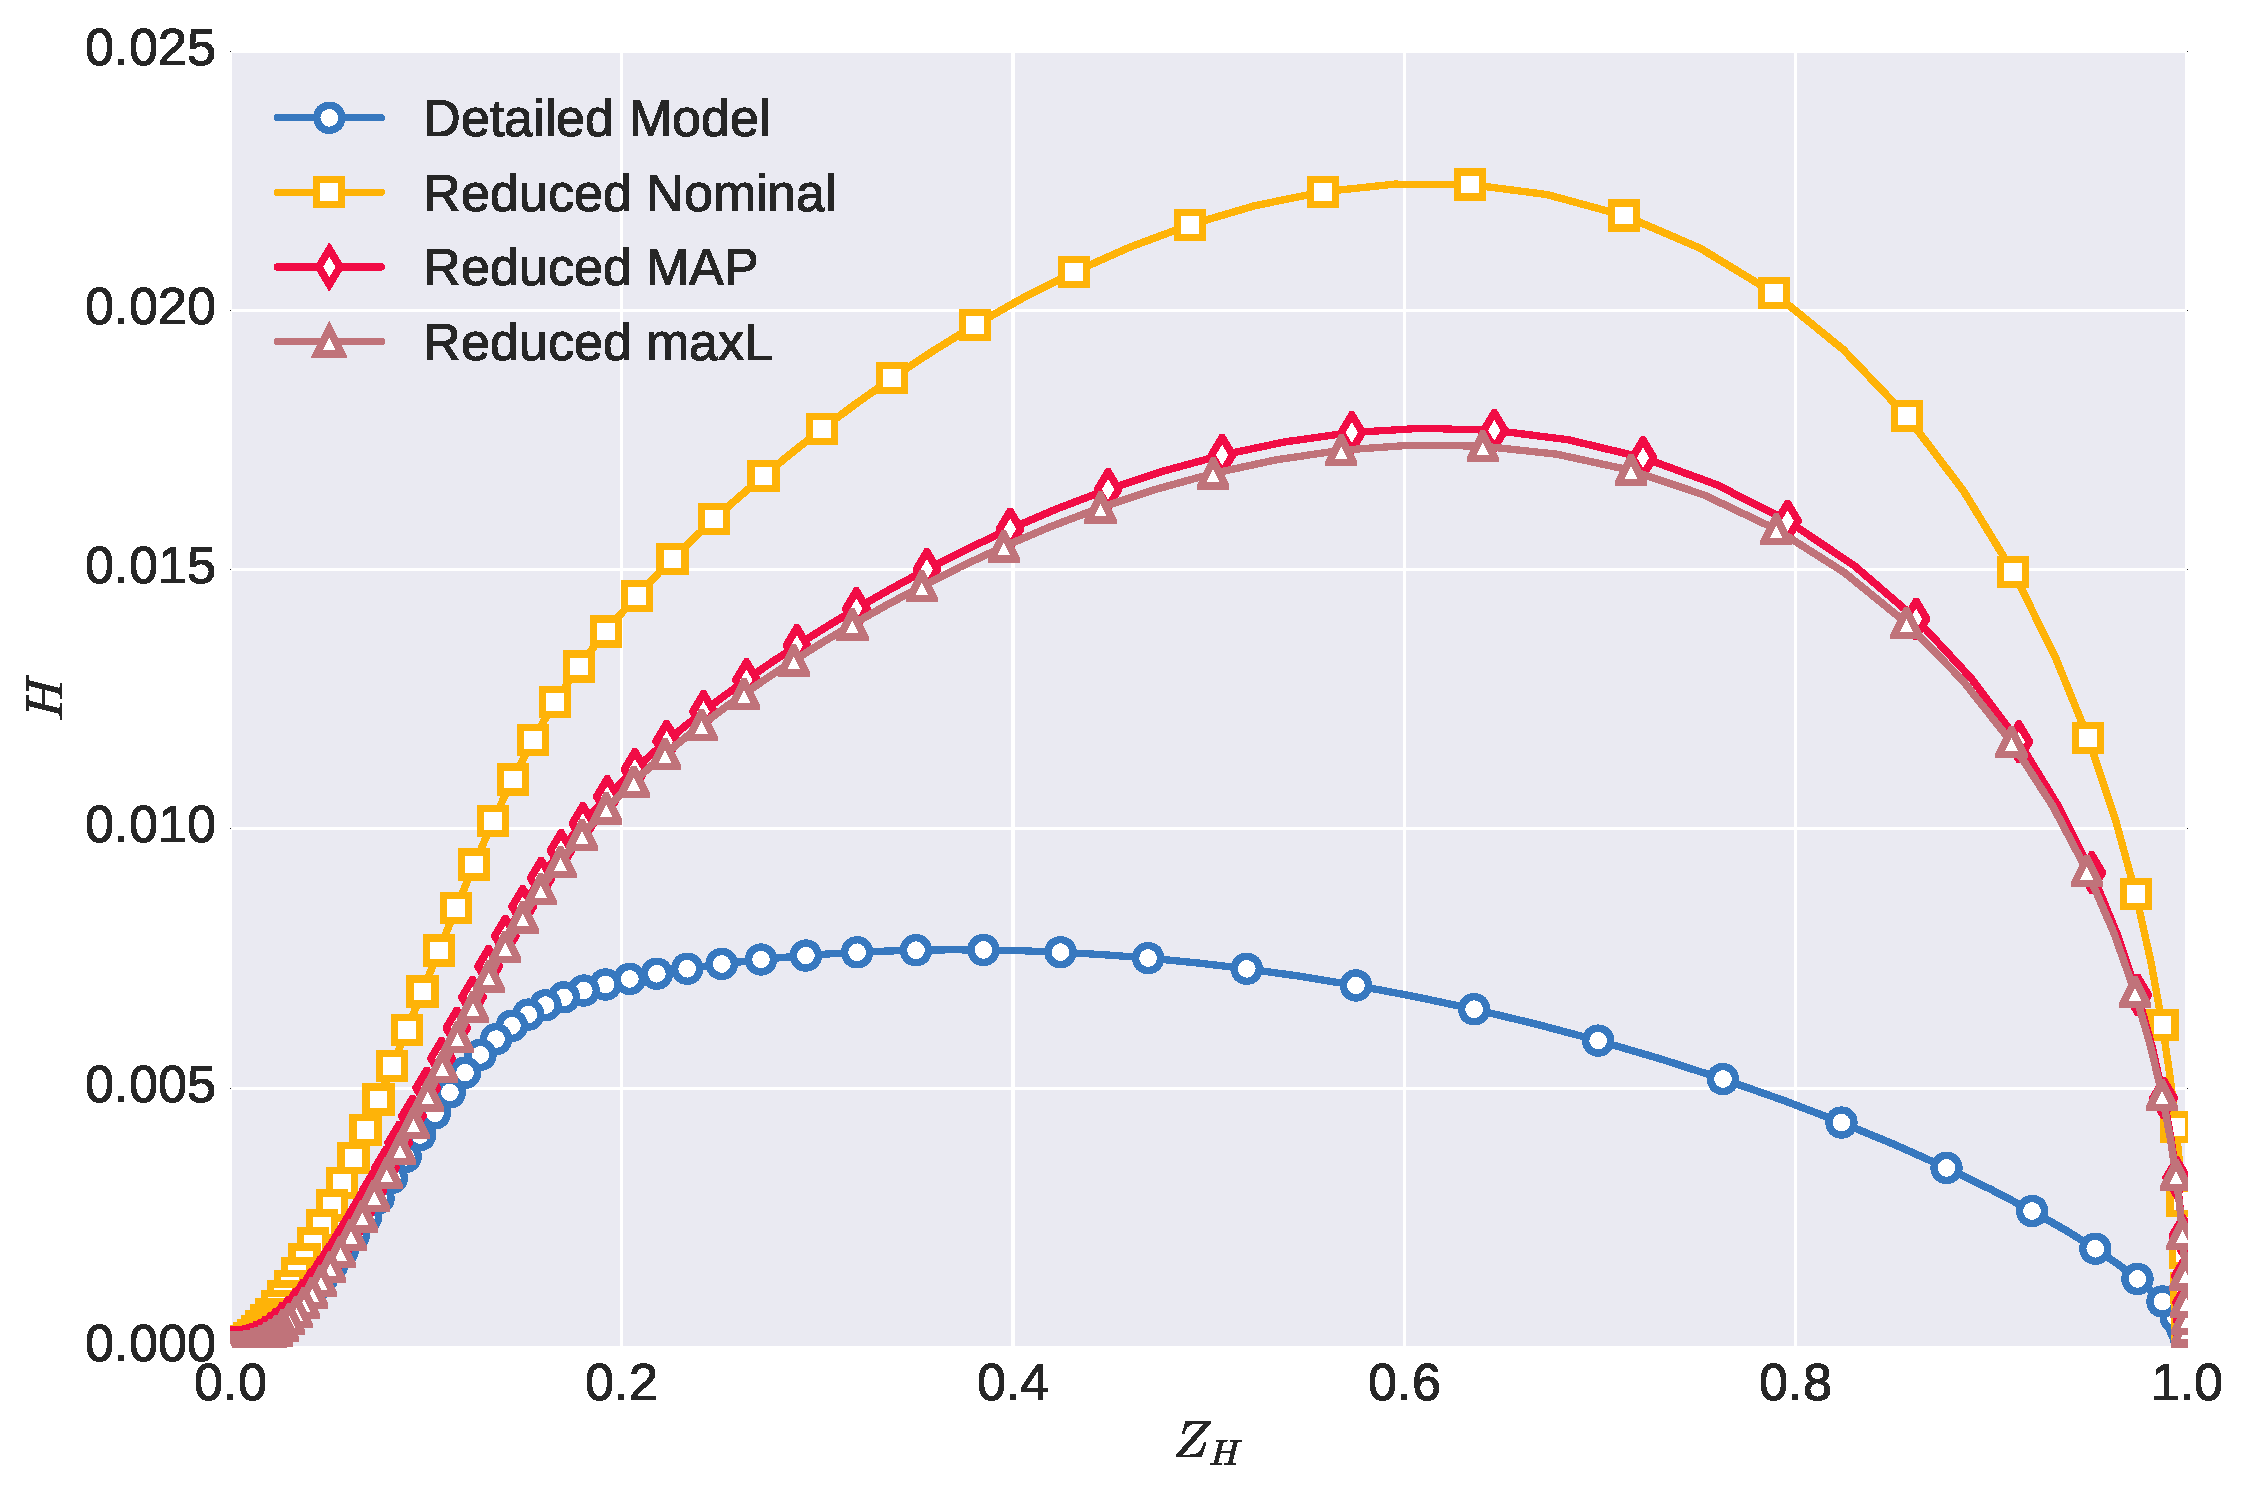
\includegraphics[width=0.7\textwidth]{/h1/dsondak/Research-Notebook/figures/2016/July/H_Z.pdf}
  \caption{Hydrogen as a function of mixture fraction.}
  \label{fig:H2_Z}
\end{figure}
\begin{figure}[h!]
  \centering
  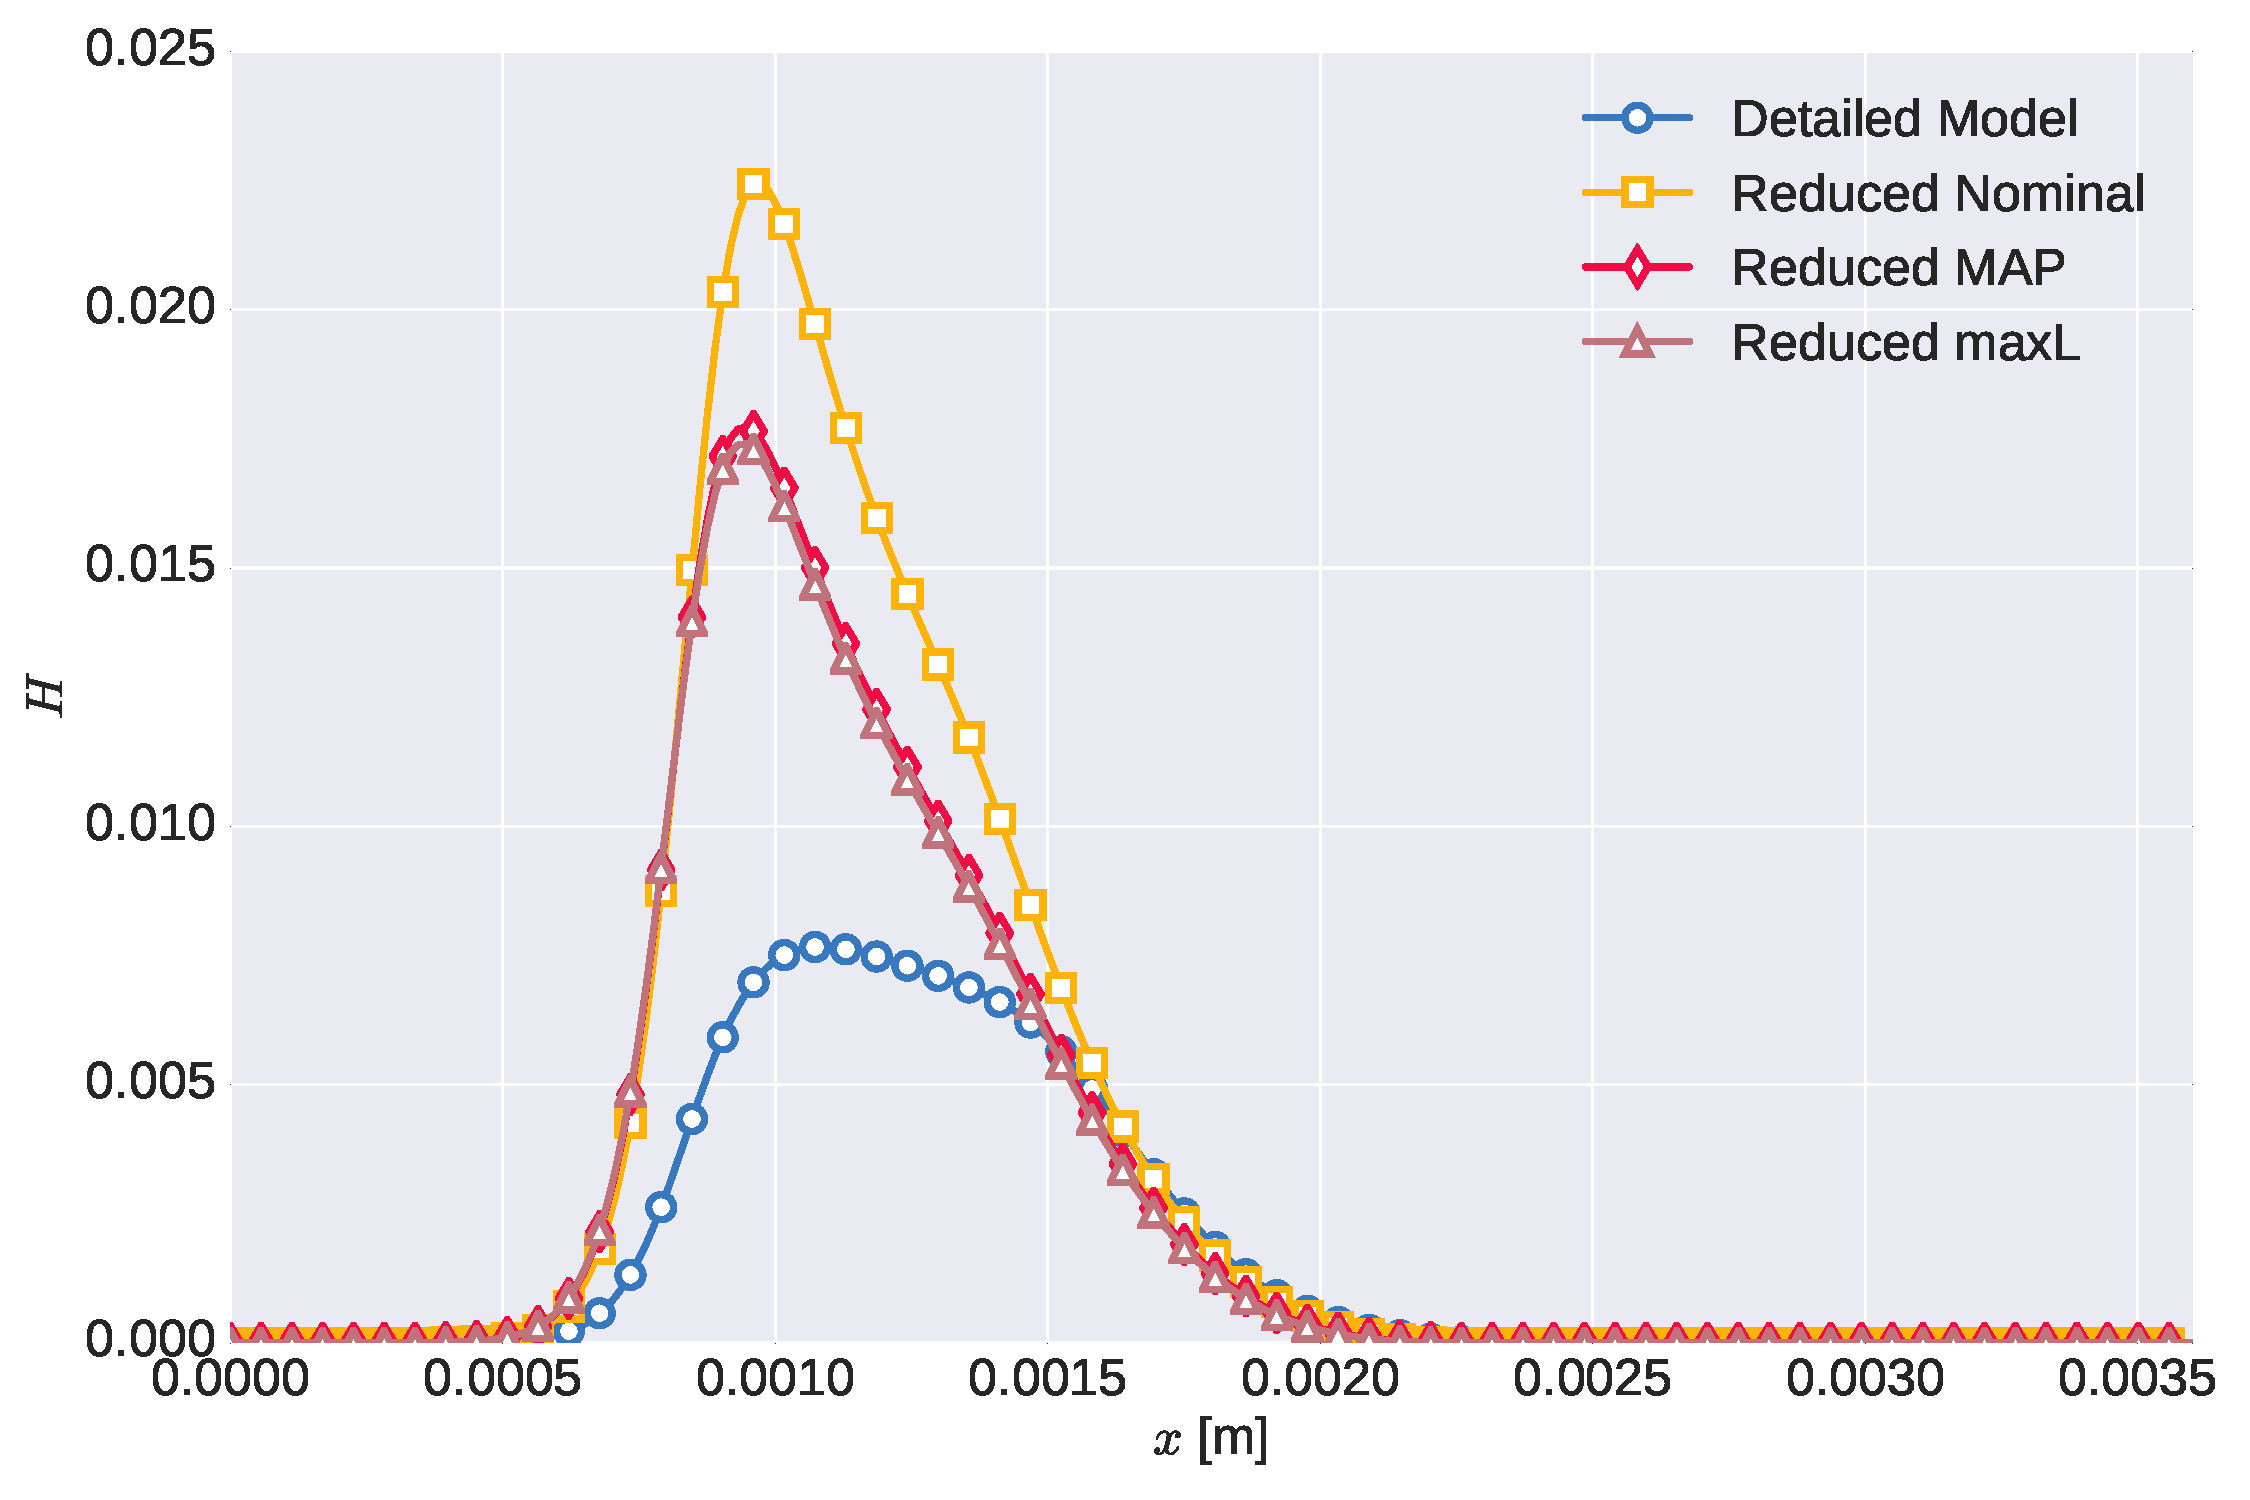
\includegraphics[width=0.7\textwidth]{/h1/dsondak/Research-Notebook/figures/2016/July/H_x.pdf}
  \caption{Hydrogen as a function of space.}
  \label{fig:H2_x}
\end{figure}
The plots of \ce{H} are clearly inadequate by almost any measure.  The plot of temperature with
mixture fraction also appears inadequate.  However, when plotting temperature with space, the results
look pretty good.  Other results indicate that some species are shifted in the domain.  That is, 
the flame location is not correct.  The concentration of \ce{HO2} is horrendously off to the point
where the reduced model predicts non-negligible concentrations while the detailed model predicts 
that \ce{HO2} is a trace species.  A few species, such as \ce{H2O}, \ce{H2} and \ce{O2} are more
or less correct as expected.  To quantify this a bit more, I will run a few samples from the chain
through the diffusion flame to see if I can put some error bars on the plots.  It will be difficult
to do this for the plots with mixture fraction since the mixture fraction will also have error bars.
However, maybe the spatial plots will show some inadequacy.

I propagated $1000$ samples through the diffusion flame and computed the mean and standard deviation
of the temperature at each grid point.  The results are plotted in Figure~\ref{fig:inad_T_x}.
\begin{figure}[h!]
  \centering
  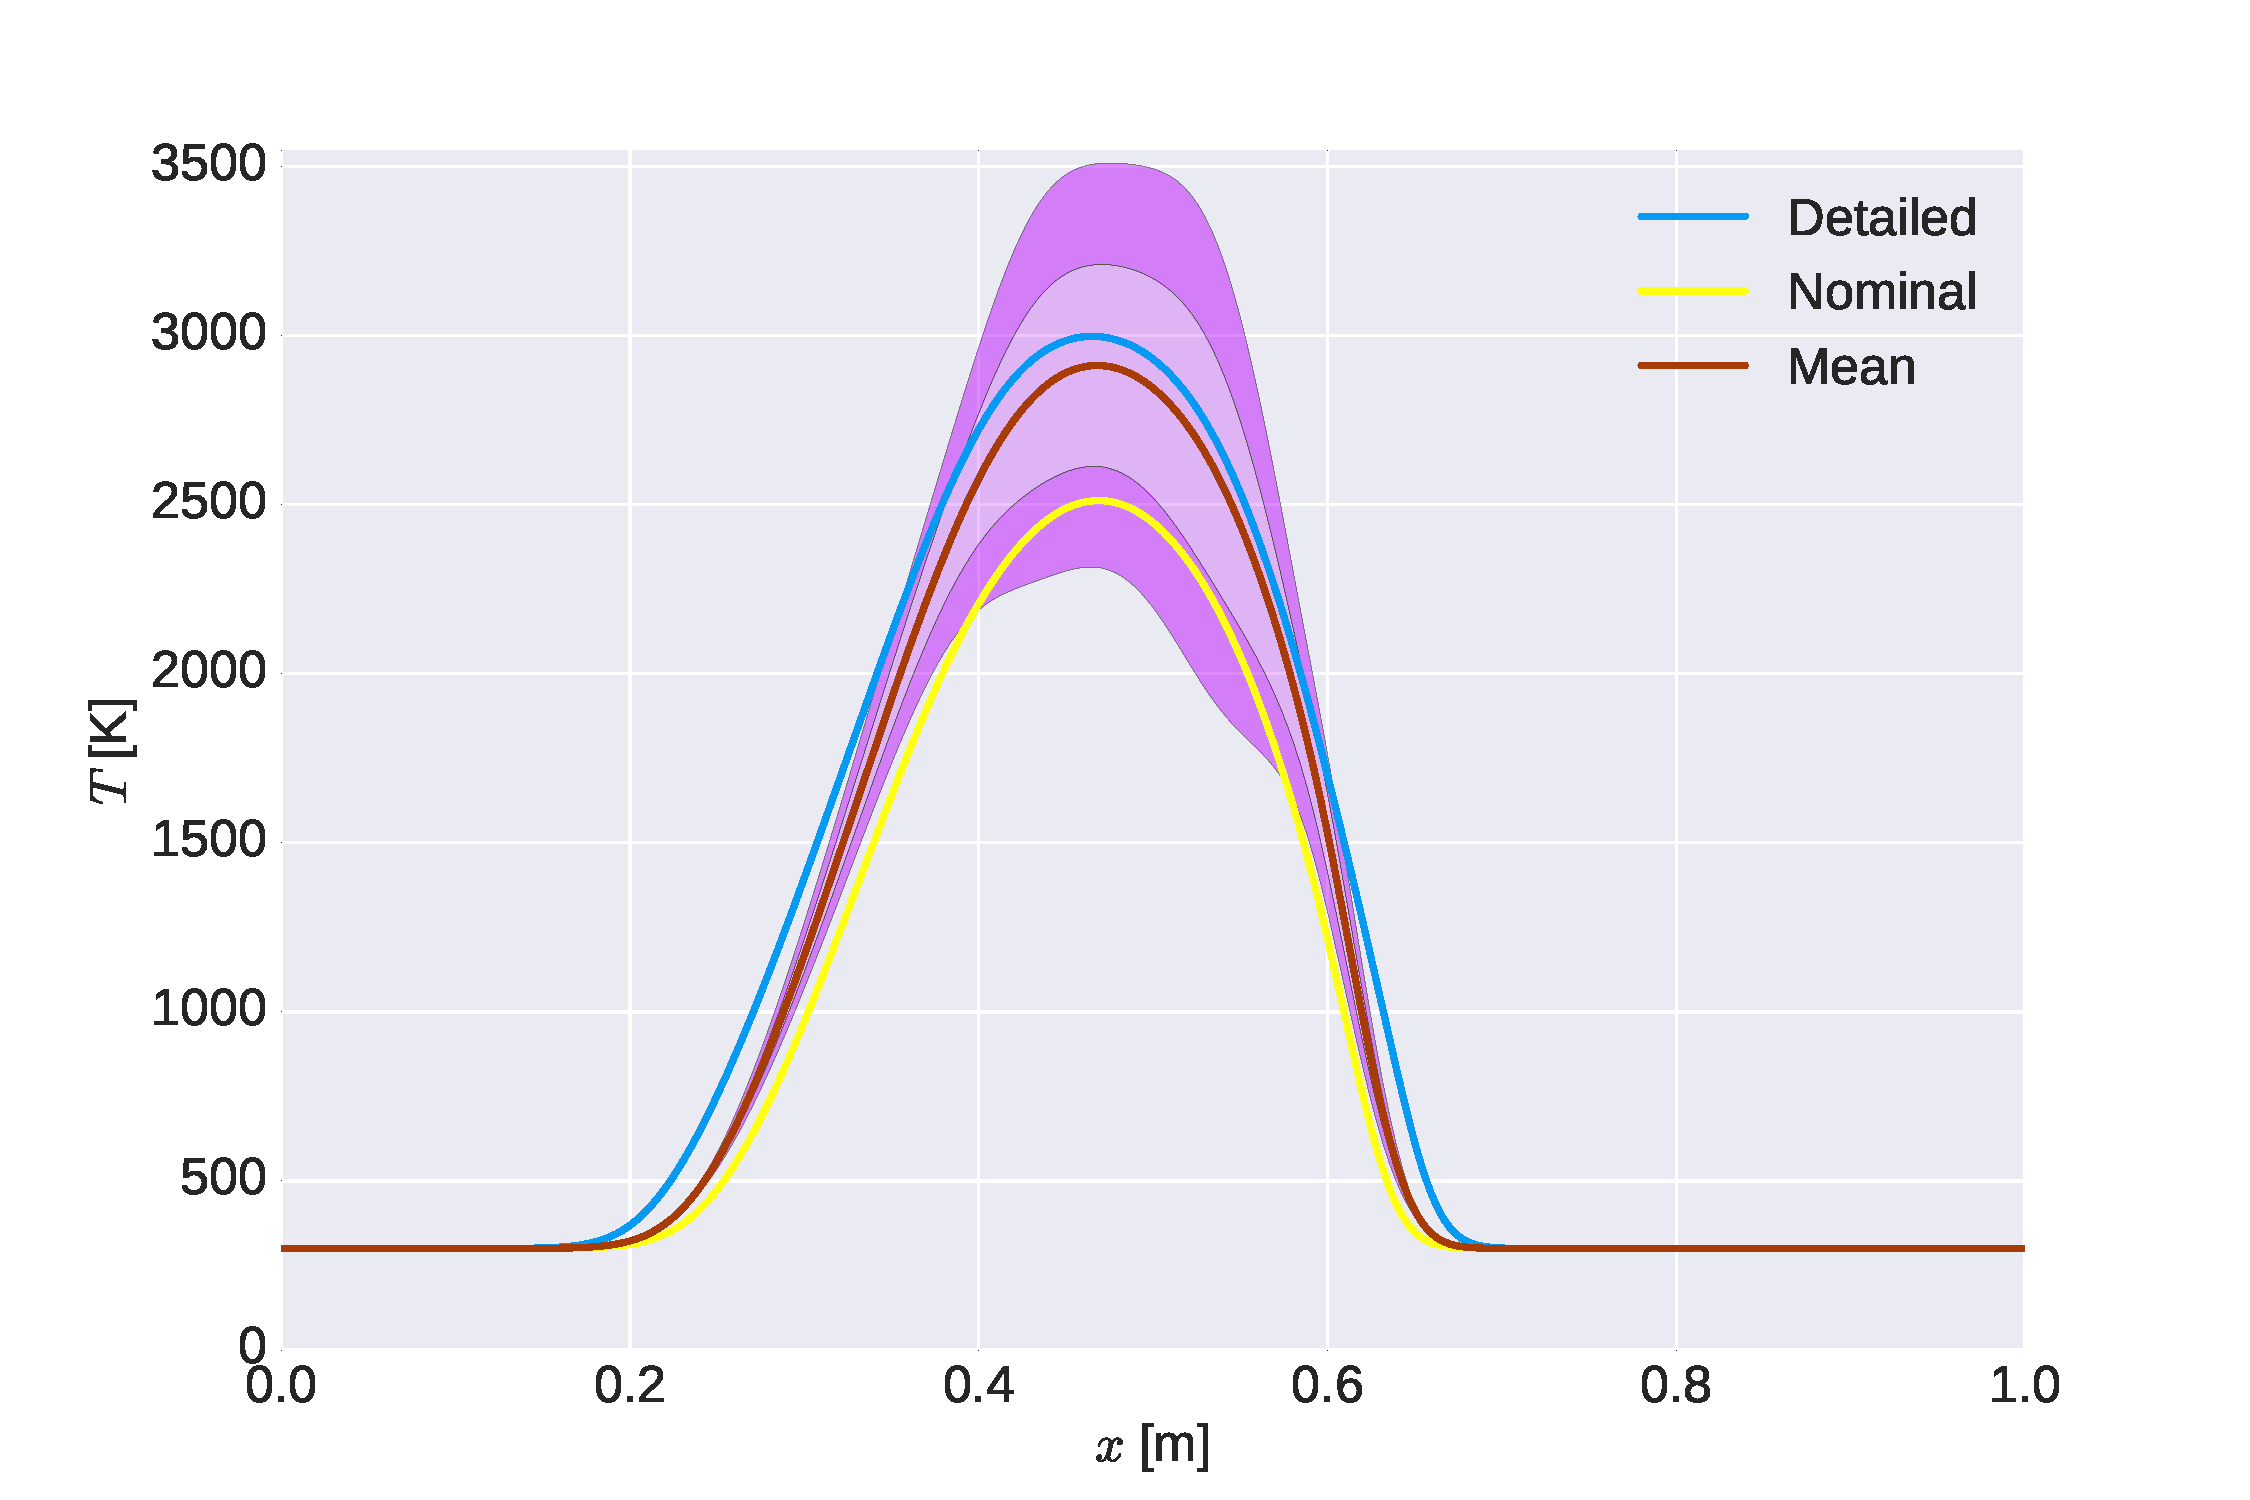
\includegraphics[width=0.7\textwidth]{/h1/dsondak/Research-Notebook/figures/2016/July/inad_T_x.pdf}
  \caption{Inadequacy in temperature profile across the diffusion flame.  Dark shading represents two
           standard deviations while light shading represents one standard deviation.  Most of the
           inadequacy occurs near the boundary of the flame.}
  \label{fig:inad_T_x}
\end{figure}
The calibrated reduced model does quite well at predicting the diffusion flame.  The main inadequacies 
are found near the boundaries of the flame.  Otherwise, the detailed model falls easily within one
standard deviation of the mean.



\end{document}

%----------------------------------------------------------------------------------------
%	LAB BOOK CONTENTS
%----------------------------------------------------------------------------------------

\labday{Thursday, 18 August, 2016}

%-----------------------------------------

\experiment{0D Reactor}
A few notes on the energy equation for the 0D reactor.  After ignoring all spatial
dependence the energy equation becomes,
\begin{align}
  \rho C_{p}\odeone{T}{t} = \dot{\omega}_{T}^{\prime} + \dot{\mathcal{Q}}.
\end{align}
Substituting for the heat release due to combustion we have
\begin{align}
  \rho C_{p}\odeone{T}{t} = -\sum_{k=1}^{N}h_{k}\lr{T}\dot{\omega}_{k} + \dot{\mathcal{Q}}.
\end{align}
Note that all quantities are on a mass basis.  The 0D reactor uses molar quantities.
\texttt{Antioch} returns mass quantities.  We need to check the units to make sure 
everything works out.

The species equation becomes
\begin{align}
  \odeone{\rho Y_{k}}{t} = \dot{\omega}_{k}.
\end{align}
Note that
\begin{align}
  \left[X_{k}\right] = \rho \frac{Y_{k}}{W_{k}} \Rightarrow \rho Y_{K} = W_{K}\left[X_{k}\right].
\end{align}
Now we have
\begin{align}
  \dot{x}_{k} = \odeone{\left[X_{k}\right]}{t} = \frac{\dot{\omega}_{k}}{W_{k}}.
\end{align}
And so the energy equation becomes
\begin{align}
  \rho C_{p}\odeone{T}{t} = - \sum_{k=1}^{N}h_{k}\lr{T}W_{k}\dot{x}_{k} + \dot{\mathcal{Q}}.
\end{align}
The specific heat is
\begin{align}
  C_{p} &= \sum_{k=1}^{N}C_{pk}Y_{k} \\
        &= \sum_{k=1}^{N}C_{pk}\frac{W_{k}}{\rho}x_{k}.
\end{align}
Then
\begin{align}
  \odeone{T}{t} = \frac{\displaystyle -\sum_{k=1}^{N}h_{k}\lr{T}W_{k}\dot{x}_{k} + \dot{\mathcal{Q}}}{\displaystyle \sum_{k=1}^{N}C_{pk}W_{k}x_{k}}.
\end{align}

%::::::::::::::::::::::::::::::::::::::::::::::::::::::::
\labday{Friday, 19 August, 2016}
%::::::::::::::::::::::::::::::::::::::::::::::::::::::::

\experiment{StochasticOP}
Trying to calibrate the stochastic operator for chemical kinetics.
Having the same problems as before with the reduced model.  Namely,
the rejection rates are simply too high and the log likelihoods are
too small.

I'm trying a few things:
\begin{itemize}
  \item Turn off stochastic operator to try to recover calibration from
        reduced model.
  \item Modify global temperature dependence to try to get better
        behavior.
  \item Played a bit with the algorithm parameters (adaptation interval
        length, etc).
\end{itemize}

Waiting to see the chains.  The global temperature dependence enters the
operator via a prefactor as
\begin{align}
  \odeone{\mathbf{x}}{t} = \mathbf{f}\lr{\mathbf{x}} + 
      g\lr{T}\left[\mathcal{S}\mathbf{x} + \mathcal{A}\lr{\mathbf{x}}\right].
\end{align}
The form that I have selected for the prefactor is
\begin{align}
  g\lr{T} = \frac{1}{2}\exp\lr{-\frac{T_{ag}}{T}}
    \left[\tanh\lr{\frac{T - T_{gi}}{\delta}} - \tanh\lr{\frac{T - T_{adi}}{\delta}}\right].
\end{align}
This introduces three new parameters to calibrate:
\begin{enumerate}
  \item $T_{ag}$, the global activation energy;
  \item $T_{gi}$, global ignition temperature;
  \item $T_{adi}$, global adiabatic temperature.
\end{enumerate}
\begin{figure}[ht!]
  \includegraphics[width=\textwidth]{August/global_T.pdf}
  \caption{Prefactor for the stochastic operator.}
  \label{fig:gofT}
\end{figure}
Figure~\ref{fig:gofT} shows the behavior of the prefactor.  The hope is that this
allows the stochastic operator to turn on and off as needed.  The Arrhenius form
basically just sets the amplitude of the prefactor and the premultiplication of 
$1/2$ just scales the hyperbolic tangents to unity (no real reason to do this
other than it helps humans see what's going on).  The smoothing factor
$\delta$ is selected to be unity.

%-----------------------------------------

%-----------------------------------------
%\end{addmargin}

\end{document}


